\documentclass[a4paper,natbib,man]{apa6}
%\documentclass[a4paper,man,natbib,floatsintext]{apa6}
%The APA6 class: http://ctan.math.utah.edu/ctan/tex-archive/macros/latex/contrib/apa6/apa6.pdf

\usepackage[english]{babel}
\usepackage[utf8x]{inputenc}
\usepackage{amsmath}
\usepackage{graphicx}
\usepackage[colorinlistoftodos]{todonotes}
\def\citeA{\citep}


% Words in text: 3309
% Words in appendices: ~700

%% User-specific lines 
\usepackage{amsmath,amssymb,amsthm}
\usepackage{soul}

%\newtheorem{thm}{Theorem}
%\newtheorem{lem}{Lemma}
%\newtheorem{dfn}{Definition}

\usepackage{amssymb,amsfonts,amsmath,amsthm}
\usepackage{mathrsfs}
\usepackage{array}
\usepackage{lineno}
\usepackage{color}
%\usepackage{ulem}

%\linenumbers

%% Macro
\def\diam{\mathrm{diam}}
\newcommand{\floor}[1]{\lfloor #1 \rfloor}
\newcommand{\ceil}[1]{\lceil #1 \rceil}
\newcommand{\one}[1]{\mathbf{1}_{#1}}
\newcommand{\vctr}[1]{\mathrm{vec}\left( #1 \right)}
\newcommand{\diag}[1]{\mathrm{diag}\left( #1 \right)}
%\newcommand{\Diag}[1]{\mathrm{Diag}\left( #1 \right)}
\newcommand{\Diag}[1]{\mathrm{Dg}\left( #1 \right)}
\newcommand{\learninggame}{learning-and-game }
\def\hsymb#1{\mbox{\strut\rlap{\smash{\Huge$#1$}}\quad}}
\newcommand{\VecSet}[2]{\mathbb{#1}^{#2}}
\newcommand{\MatSet}[2]{\mathbb{#1}^{{#2}\times{#2}}}
\newcommand{\MatSets}[3]{\mathbb{#1}^{{#2}\times{#3}}}
\newcommand{\Encode}[2]{\mathcal{C}_{#1,#2}}
\newcommand{\Simplex}[1]{\mathbb{S}^{#1}}
\newcommand{\SimMat}[1]{\mathbb{S}^{#1 \times #1}}
\newcommand{\SimMats}[2]{\mathbb{S}^{#1 \times #2}}

\newcommand{\Trans}[2]{#1^{(#2)}}
\newcommand{\TransBlock}[3]{#1_{#3}^{(#2)}}
%\newcommand{\TransBlockVec}[4]{#1_{#3, #4}^{(#2)}}
\newcommand{\TransBlockVec}[4]{#1_{N(#3-1) + #4}^{(#2)}}

\newcommand{\TransBlockNo}[2]{#1_{#2}}
\newcommand{\TransBlockVecNo}[3]{#1_{#2, #3}}
\newcommand{\zero}[1]{\mathbf{0}_{#1}}
\newcommand{\rank}[1]{\text{rank}\left(#1\right)}

%% For the application
\newcommand{\dd}[0]{\text{d}}

%\newcommand{\argmax}{\mathop{\rm arg~max}\limits}
%\newcommand{\argmin}{\mathop{\rm arg~min}\limits}
\DeclareMathOperator*{\argmin}{arg\,min} %argmin
\DeclareMathOperator*{\argmax}{arg\,max} %argmax


%\newtheorem{thm}{Theorem}[section]
\newtheorem{thm}{Theorem}[]
%\newtheorem{cor}[thm]{Corollary}
\newtheorem{prop}{Proposition}
%\newtheorem{lem}[thm]{Lemma}
\newtheorem{lem}[]{Lemma}
%\newtheorem{def}[thm]{Definition}
\newtheorem{definition}[]{Definition}
\newtheorem{cor}[]{Corollary}

%\newcommand{\SH}[1]{\textcolor{red}{#1}}
%\newcommand{\GK}[1]{\textcolor{orange}{#1}}
\newcommand{\SH}[1]{#1}
\newcommand{\GK}[1]{#1}

%\title{Active learners can learn what simple samplers cannot: A Zipf-distributed vocabulary from limited data} 
\title{Active learning expedites cross-situational word learning--even under Zipfian distributions}
%\title{A theoretical analysis of active cross-situational word learning under Zipfian distributions}
\shorttitle{Active word learning}
\author{Shohei Hidaka$^1$, Takuma Torii$^1$, and George Kachergis$^2$}
%\author{Anonymous author(s)}
\affiliation{$^1$School of Knowledge Science, Japan Advanced Institute of Science and Technology, Nomi, Ishikawa, 923-1292, Japan and $^2$Department of Psychology, Stanford University, Stanford, CA, 94305, USA}
%\affiliation{Affiliation}

% Brief articles reporting original empirical findings, major theoretical advances or crucial developments that warrant rapid communication to the scientific community - limit 3000 words including abstract (excluding references)
% http://app.uio.no/ifi/texcount/online.php  2940 words as of 9/11/18 (+122 in captions)

%\keyword{Keywords: Word learning; Active learning; Zipf’s law; Fast mapping; Linear programming; Word frequency} % duplicate of \keywords{} below; apa6 has no \keyword command

\authornote{The authors have no conflict of interest to declare.}

% abstract updated, ~280 words
\abstract{
Children learn thousands of words in the first several years of life, inspiring many theoretical and empirical studies of the mechanisms and pace of word learning.
Past mathematical analyses have asked how long it should take a child to build an adult-sized vocabulary if words are encountered via random sampling, and concluded that this simple process can succeed in a plausible amount of time--but only under the simplifying assumption that every word is equally likely to be encountered.
We show that this optimistic conclusion depends heavily on that assumption: under the more realistic, highly-skewed (Zipfian) word and referent frequency distributions observed in child-directed speech and in real-world scenes, random sampling requires an implausibly large number of learning episodes.
We then ask whether a learner (or caregiver) who can influence which words and referents co-occur, rather than simply encountering them at random, can close this gap.
Using both mathematical analysis and simulation--including three more realistic incremental learners that do not assume words are learned in a single exposure--we show that such active learners acquire Zipfian vocabularies substantially faster than passive learners exposed to the same random samples, with the size of the advantage depending on how idealized the learning scenario is, and growing severalfold between a functional and a fully complete vocabulary.
This advantage does not depend on an idealization of perfect, unlimited memory for tentative word-referent guesses: it survives, and even strengthens, once a cognitively realistic forgetting mechanism is introduced.
These results suggest that the statistical structure that children (or their caregivers) impose on everyday learning situations, rather than sheer exposure alone, may be an important piece of the explanation for how children learn vocabulary as quickly as they do.}

\keywords{Word learning; Active learning; Zipf’s law; Fast mapping; Linear programming; Word frequency}

\begin{document}

\maketitle

\section{The remarkable pace of word learning}

Language acquisition proceeds quickly in young children, who within their first year learn the sounds of their language \citep{Kuhl:1992}, begin segmenting speech \citep{Saffran:1996} and even produce their first words \citep{Hulit:2002}.
Under the common assumption of roughly 8 hours of daily word-learning opportunity, reaching the oft-cited target of 60,000 words by 18 years of age \citep{Bloom:2000} implies learning a new word every learning hour, on average, for 18 years.
This pace seems remarkable, given the storied complexity of the learning environment: a given word could refer to any of infinite possible meanings in any given situation \citep[cf.][]{Blythe:2016}.

Table~\ref{tab-vocab-benchmarks} summarizes representative vocabulary-size estimates across this developmental window, drawn from several sources that differ in methodology (comprehension vs.\ production, different instruments) and so are not directly comparable to one another; the trajectory they share is a rapidly accelerating one--from single digits of words in the first year to several hundred by two, roughly a thousand by three, and at least ten thousand comprehended words by five \citep{Shipley:2015,Anglin:1993}--well before the 60,000-word, 18-year target most of vocabulary growth still lies ahead.

\begin{table}[h]
\centering
\caption{\label{tab-vocab-benchmarks} Representative vocabulary-size estimates across development. Comprehension and production are measured differently and are not directly comparable to one another; see cited sources for instrument details.}
\small
\begin{tabular}{@{}p{2.2cm}p{2.2cm}p{3.0cm}p{5.5cm}@{}}
\hline
Age & Estimate & Metric & Source \\
\hline
12 months & $\sim$7 words & Production (CDI) & \citep{Frank:2017} \\
18 months & 50--120 words & Production (CDI) & \citep{Frank:2017} \\
18 months & 100--150 words & Comprehension & \citep{Hulit:2002} \\
24--30 months & 220--530 words & Production (CDI) & \citep{Frank:2017} \\
3 years & $\sim$1,000 words & Comprehension & \citep{Hart:1995} \\
5 years & $\geq$10,000 words & Comprehension & \citep{Shipley:2015} \\
18 years / adult & $\sim$60,000 words & This paper's primary target & \citep{Bloom:2000} \\
\hline
\end{tabular}
\end{table}

Throughout this paper we follow prior theoretical work in analyzing the feasibility of this 18-year, 60,000-word target \citep{Blythe:2010,Vogt:2012,Blythe:2016}, since it is the estimate against which our results are most directly comparable.
It is worth flagging up front, however, that this target describes vocabulary growth across childhood as a whole, including the school years; the pre-literacy period our spoken, caregiver-mediated sampling models most directly address reaches only around 10,000 comprehended words by age five (Table~\ref{tab-vocab-benchmarks})--an order of magnitude short of the full target, and before written text, with its different frequency distribution and sampling process, becomes an increasingly important source of new vocabulary.
We retain the 60,000-word, 18-year benchmark throughout for comparability with prior work, and return to what this scoping implies for our conclusions in the Discussion.

How might young children tackle the daunting problem of mapping words to referents at this pace?


A variety of heuristics and mechanisms are thought to help learners mitigate referential uncertainty, and empirical studies have shown that young children can take advantage of many of them in the laboratory. 
For example, children can leverage social cues \citep{HirshPasek:2000}, can learn a word from a single informative instance \citep[i.e., {\em fast-map};][]{Carey:1978,Spiegel:2011}, tend to assume words refer to whole objects \citep{Macnamara:1972}, \GK{and are biased to form mutually exclusive word-referent mappings \citep{Merriman:1989}}. 
These heuristics are assumed to aid the process of {\it cross-situational learning}: acquiring words by accumulating evidence for meanings across multiple contexts--an ability demonstrated in the lab by infants and adults \citep{Smith:2008vg,Yu:2007}. 
However, determining the relative contributions of these myriad heuristics to naturalistic cross-situational word learning remains a challenge, \GK{despite their inclusion in various computational models of word learning, both because such models are primarily applied to experimental settings, and because the complexity and structure of real-world learning environments is largely unknown \citep[though see][]{Smith:2018,Suanda:2018,Clerkin:2017}.}

\GK{Moreover, there is disagreement over the basic mechanisms governing word learning: hypothesis-testing models view the problem as one of inference in which the learner may propose and test a single mapping for each word and referent \citep[e.g.,][]{Trueswell:2013}, while associative models gradually accumulate noisy knowledge traces representing graded links between multiple words and referents \citep[e.g.,][]{McMurray:2012,Kachergis:2012gi}.
Both types of models can implement fast mapping, mutual exclusivity, and other heuristics, and although they are not always equivalent, it has been shown that these models may often mimic one another's behavior \citep{Yu:2012hyp}, making it difficult to choose a general approach to modeling word learning. 
Nonetheless, it has proven useful to test the overall strength of simple learning mechanisms in idealized simulations of the language learning environment in order to explore the long-term behavior and plausibility of such mechanisms for learning an adult-sized (60,000-word) vocabulary \citep{Blythe:2010,Vogt:2012,Blythe:2016}.}

\subsubsection{Distributions of words and referents}

Past analyses have generally modeled word learning as a process that randomly samples a single word together with a situation containing a target meaning and, often, several distractor meanings.
For example, \cite{Blythe:2010,Blythe:2016} analyzed an idealized learning model that learns each word on its first sample (i.e., {\it fast-mapping}, or one-shot learning), in order to estimate the fastest possible learning rate needed to learn a full-sized vocabulary.
Because fast-mapping succeeds the instant the target word and its referent co-occur, distractor meanings play no role in this model: the learner simply needs the correct word-referent pair to appear, so the relevant distribution is the frequency with which each word (equivalently, its unique referent, under a mutually-exclusive word-referent mapping) is sampled.
Under the simplifying assumption that this word frequency (WF) is uniformly-distributed (Figure~\ref{fig-overview}, top left), \cite{Blythe:2010}'s mathematical analysis of the model showed that a cross-situational learner is likely to learn an adult-sized vocabulary (i.e., $\sim60,000$) words after only $\sim940,000$ samples, a number of spoken words that is well within the bounds of human life experience, requiring roughly 142 learning instances per day for 18 years. %
Blythe \textit{et al}.'s analytical estimate has been treated as a theoretical implication that learning via independent fast-mapping of words is sufficiently powerful to be a model of child word learning.
\cite{Blythe:2010} also considered a Zipf-distributed word distribution, finding that it should be slower by a factor that depends on the size of the to-be-learned vocabulary (11.58 for 60,000 words, so 10.9 million). % 940000*11.58 = 10,885,200;  -- Blythe et al. 2010's upper bound based on Hart and Risley (2003): 2,100 words per hour, 14 h of exposure per day for 18 years = 2100 * 14 * 365 * 18 = 193,158,000
% realistic bound: 1000 * 14 * 365 * 18 = 91,980,000

A separate question is what happens when situations contain multiple candidate meanings whose \textit{identities}, not just the target word's frequency, matter to the learner--for instance, a learner who must eliminate distractors across several exposures rather than fast-mapping in one shot.
Analysis of egocentric views from head-mounted cameras on 8- to 10-month-old infants shows a right-skewed frequency distribution of the objects children actually attend to \citep{Clerkin:2017}, suggesting that the meanings available in naturalistic learning situations are themselves Zipfian, independent of how often any given word is spoken.
\cite{Vogt:2012} modeled exactly this scenario: words and their possible (distractor) meanings were both drawn from Zipfian distributions, and because his learner narrows down a word's referent by eliminating distractors across episodes (rather than fast-mapping), a highly-frequent distractor meaning tends to co-occur with the target on every exposure, slowing learning even further. Using Monte Carlo simulation, \cite{Vogt:2012} found that learning times increase super-exponentially as a function of the ratio of the context size ($C$) to the number of incidental meanings ($M$), with human-scale learning only plausible for ratios of $C/M \leq .1$--i.e., situations in which fewer than a tenth of all possible meanings are plausible candidates.
This distractor-elimination slowdown is conceptually distinct from the slowdown we analyze in the next section: ours arises purely from a nonuniform \textit{word} frequency distribution under fast-mapping, where distractor identities are irrelevant by assumption, whereas Vogt's arises from the composition of the distractor set under a different (elimination-based) learning mechanism. We return to the role of situation composition--which becomes central rather than incidental--when we consider active learners in the Active learning section below.


\subsubsection{Active learning}

In stark contrast to these sampling models of word learning, which treat the learner as a passive recipient of externally-determined input, a growing body of work in neuroscience and cognitive science emphasizes that learners actively shape what they attend to and experience, driven by curiosity and the pursuit of informative input \citep{gottlieb2018towards}.
Infants and young children direct their gaze, reach, and requests toward informative objects and events, and structure joint-attention episodes with caregivers in ways that concentrate a single object in view at a time \citep{Yu:2009active}, with young children also showing measurable benefits from being given active control over their own learning \citep{Partridge:2015}.
Analogous benefits of self-directed sampling have been demonstrated in adult word learners given explicit control over which items to study \citep{Kachergis:2013,zettersten2021sampling}.
Reviewing this literature, \cite{Foushee:2023} argue more broadly that language development itself should be reconceived around an actively-learning child--one who seizes learning opportunities and selects informative input--rather than the traditionally-assumed passive recipient of adult-directed speech.
These findings raise the possibility that active selection of learning situations--rather than passively-sampled input alone--may be part of how children (or their caregivers) overcome the slow learning implied by the analysis above.


\subsection{The present study}

The present study reinspects independent fast-mapping under a more realistic power-law word frequency distribution (WFD) that is characteristic of natural language \citep{Zipf:1949}.
Our new mathematical analysis implies that the learning rate of independent fast mapping is quite sensitive to nonuniform distributions of words and referents.
Critically, under a Zipfian word frequency distribution, even fast-mapping--the most generous passive learning scheme, since it requires only a single co-occurrence to learn a word--implies an implausibly large number of learning episodes to acquire 60,000 words within 18 years.
Intuitively, the difficulty with quickly learning a long-tailed distribution under random sampling is that a learner must wait a very long time to hear the large proportion of low-frequency words.
This is a useful diagnostic precisely because fast-mapping is the best case for passive, independent word learning: if even this idealized scheme implies an implausible number of samples, it suggests that random sampling alone is an incomplete account of how children learn a Zipfian vocabulary, whatever the details of how any individual word is learned.
We confirm that simulated learning from the Zipfian WFD in the CHILDES database \citep{MacWhinney1990}, a corpus of child-directed speech, is similarly slow, and--going beyond fast-mapping--show with simulation that a more realistic incremental learner, which accumulates evidence for a word-referent mapping across multiple exposures rather than guessing correctly on the first one, shows the same qualitative pattern (see the Incremental active learning section).

% Vogt:2012 / Blythe:2010 model assumptions (as Vogt wrote): (a) a word is always exposed in a situation where its meaning is present, (b) each word and situation are perceived without errors, (c) all situations have the same number of distinct incidental meanings, (d) all meanings are given, so there is no need for categorization, and (e) the lexicon is unambiguous.

\begin{figure}[h]
\begin{center}
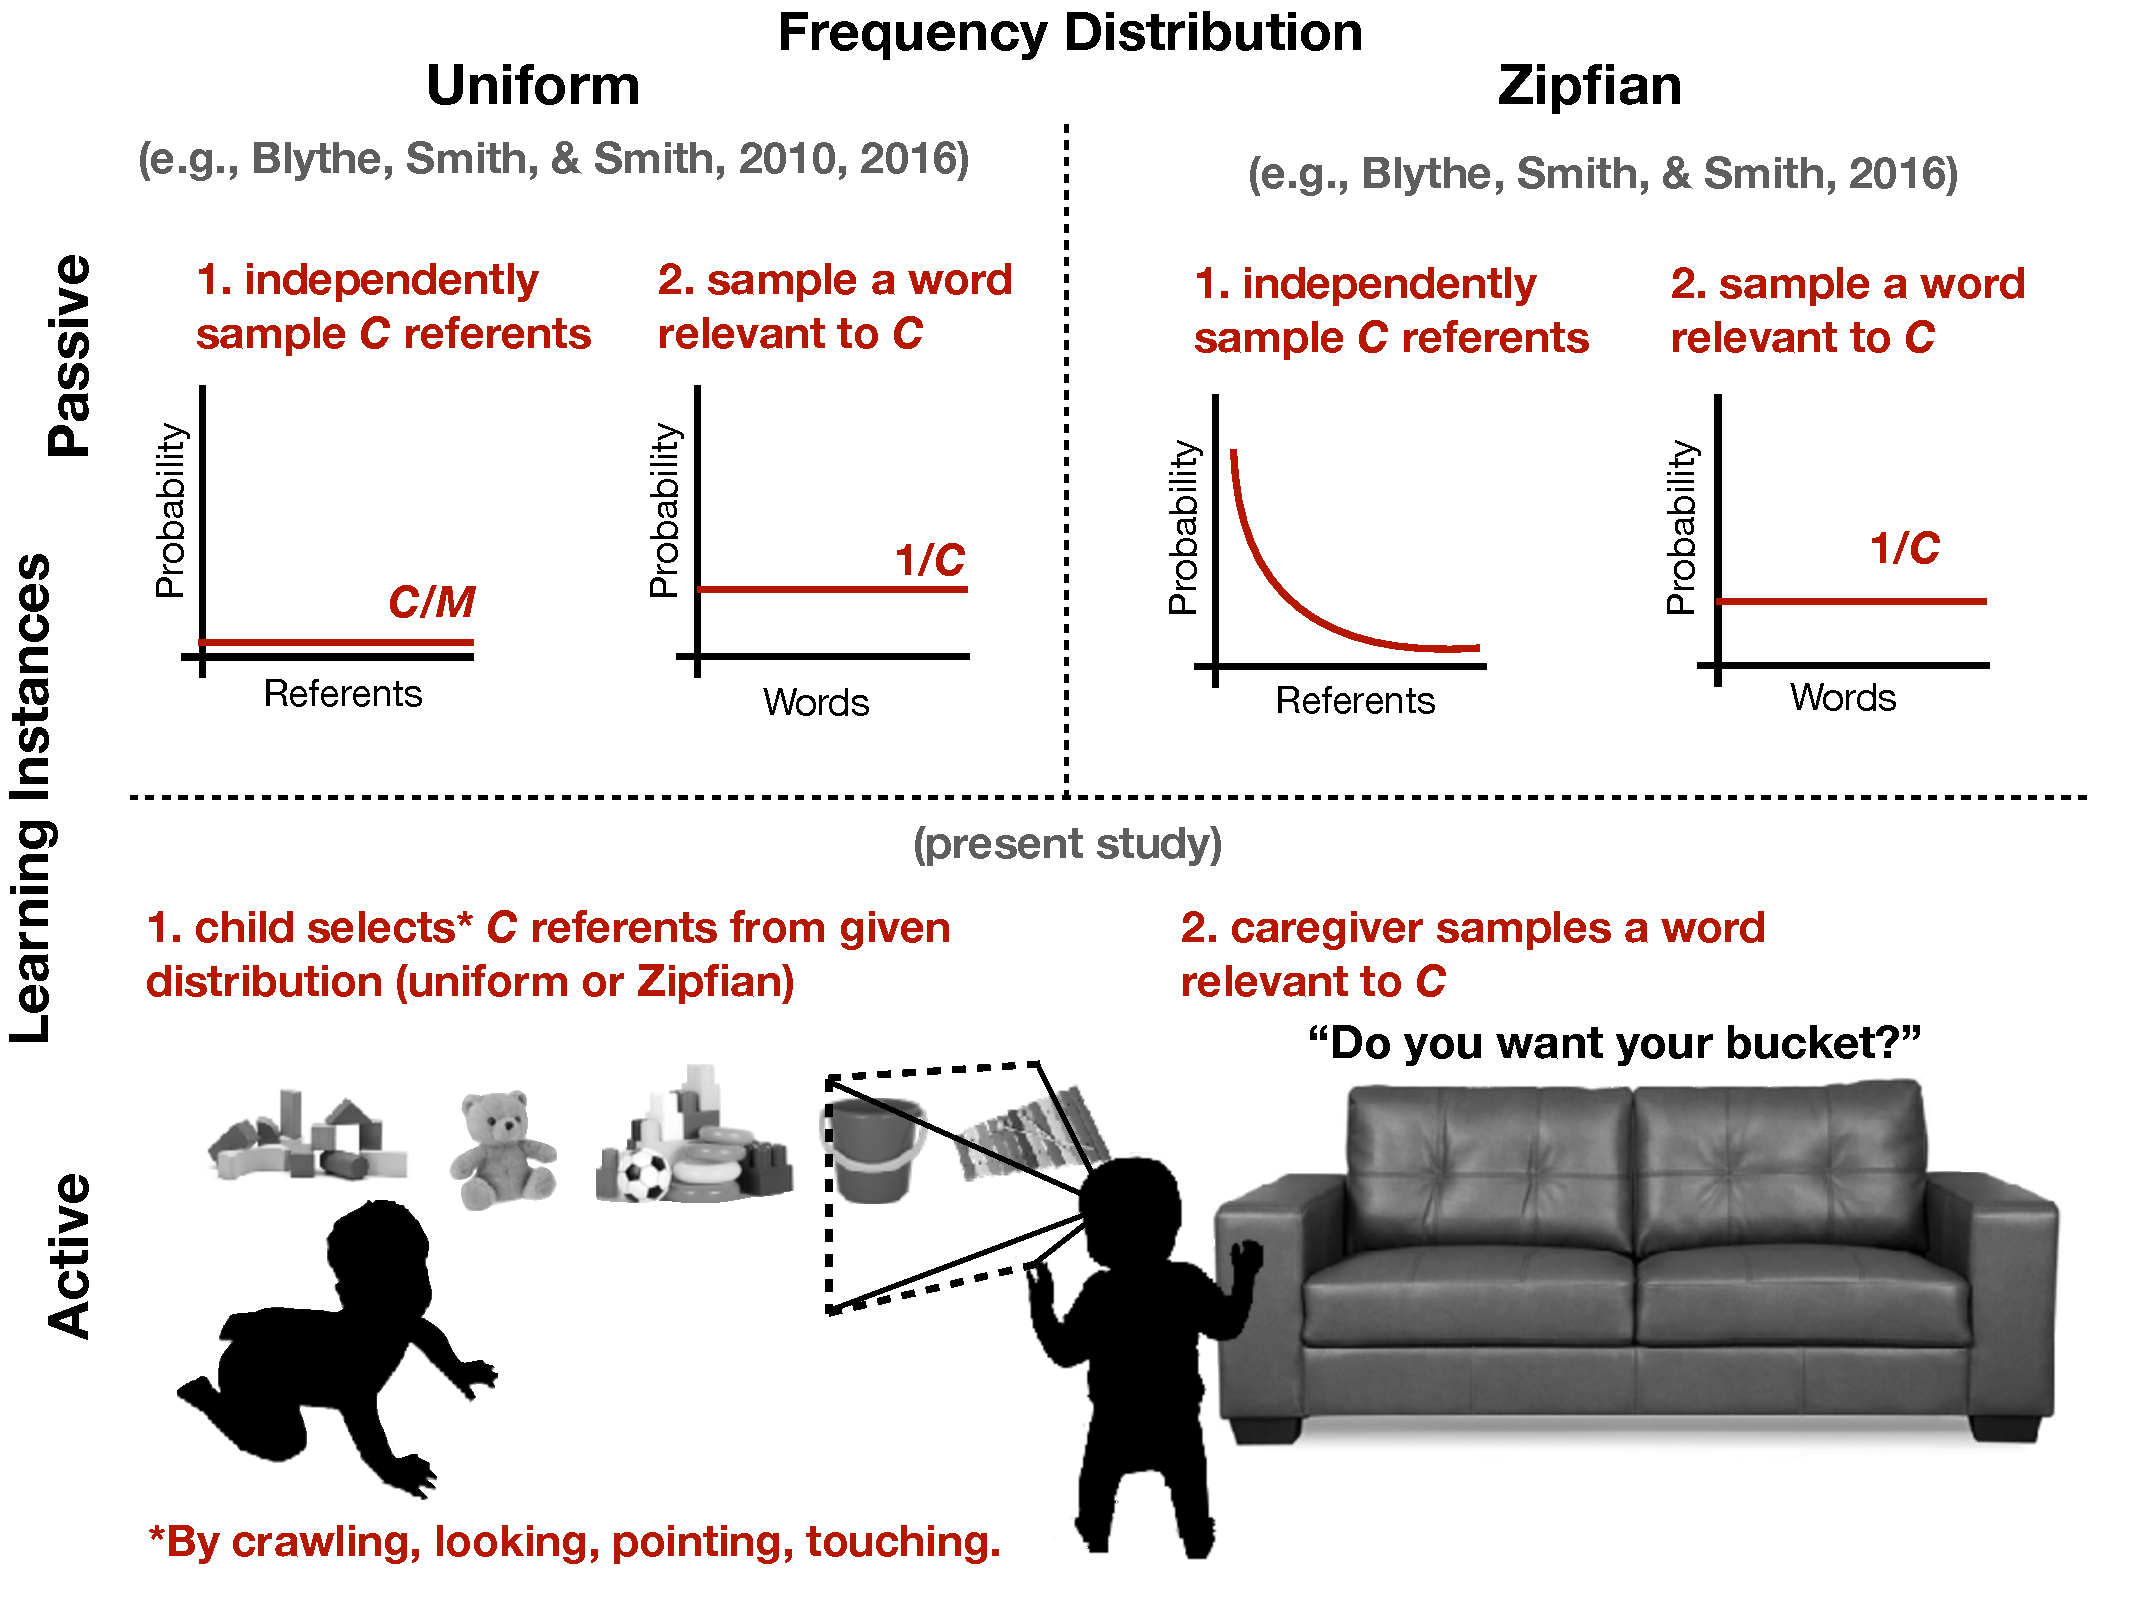
\includegraphics[width=\linewidth]{fig1-distros_vs_active_v2}
\caption{\label{fig-overview} 
  Previous research considered passive learning from independent random samples from uniform (top left) or Zipfian (top right) word and referent (i.e., meanings $M$) frequency distributions. The present work shows that passive learning from a Zipfian word and referent distribution requires an implausibly large number of samples, and explores active learning--a general scheme by which the infant (or caregiver) chooses the situation (i.e., context $C$) from which they will learn (bottom)--as a candidate source of the additional speed children's learning requires. }
\end{center}
\end{figure}

Given the difficulty of learning naturally-occurring Zipfian WFDs even with the power of fast-mapping, and motivated by the active and curiosity-driven learning literature reviewed above, we explore an extension of the word learning problem in which the learner is not simply a passive recipient of randomly-selected words and referents \citep[as in][]{Blythe:2010,Vogt:2012,Blythe:2016}, but instead has some ability to structure the situations from which they will learn: choosing which referents to bring into a situation, from which a caregiver then selects a target referent to name (see Figure~\ref{fig-overview}).
% mention active learning in education (e.g., Montessori; Nolan, A., Kilderry, A., and O'Grady, R. (2006). Young children as active learners, Early Childhood Australia, Watson, A.C.T.)
Our analysis shows that this form of active learning yields substantial speedups over passive random sampling--in some cases bringing learning times within a plausible range for real-world timescales--even under a long-tailed Zipfian WFD, though the size of the speedup depends on how much of the learning process is idealized (see the Active learning section and the Incremental active learning section).

In summary, this paper offers five main contributions:
\begin{itemize}
\item {\bf A general analytical bound.} We derive a closed-form bound on fast-mapping time for an arbitrary word frequency distribution, not only the uniform and Zipfian cases analyzed previously, and validate it against two independent corpora (CHILDES child-directed speech and Google Books).
\item {\bf Formal and empirical characterization of active learning's ceiling.} We characterize the maximum benefit active control over learning situations can confer, evaluated using real object-scene co-occurrence statistics from the SUN database, and test a more realistic online learner that must estimate this structure from experience rather than know it in advance.
\item {\bf Three incremental learning mechanisms.} We simulate three distinct mechanisms that require multiple exposures rather than a single co-occurrence--each embodying a different account of how evidence for a word's meaning accumulates--crossed with active and passive selection of both target words and their accompanying distractors.
\item {\bf The advantage depends on the completion target.} We show that the size of the active-learning advantage is not a single number: it grows severalfold between a functional (50--90\%) and a fully complete (99\%) vocabulary.
\item {\bf The advantage survives, and strengthens under, forgetting.} We test whether this advantage depends on an idealization of perfect, unlimited memory for tentative guesses, and find that it does not merely survive a more cognitively realistic forgetting mechanism, but strengthens under it.
\end{itemize}

% Vogt:2012 - Fig. 4 shows that when C/M=0.1, the learning time t~=10^8, which in 18 years would amount to 15,221 words per day. When C/M 1⁄4 0.2, however, the learning time t~=2.9x10^9, which comes to about 441,400 words per day in 18 years. Assuming the upper bound of the number of words that parents are estimated to speak to their children (Hart & Risley, 2003), when hearing 2,100 words for 7.2 h per day, learning 60,000 words in 18 years is feasible with XSL, if C/M 1⁄4 0.1. However, children would require 210 h of input per day if C/M=0.2. Clearly, the former situation is plausible, and the latter is not.

\section{Methods}

The sections that follow analyze several related models, which can be hard to keep straight without a shared vocabulary and a concrete example to anchor the notation. This section lays out both, and previews how the pieces fit together.

\subsection{Shared ingredients}
Every model in this paper shares the same basic scenario. There are $W$ words to be learned, and--for simplicity, following \cite{Blythe:2010}--exactly $W$ referents (meanings), with each word paired with one and only one referent (a {\it mutually-exclusive} lexicon; we return to this simplifying assumption, including the role of synonymy, in the Discussion). The learner experiences a sequence of {\it episodes}. In each episode, they encounter a {\it situation}: a spoken word, together with a set of candidate referents present in the scene, one of which (the {\it target}) is the word's true referent and the rest of which (if any) are {\it distractors}.

Two things can vary independently across the models we analyze:
\begin{itemize}
\item {\bf How situations arise.} A {\it passive} learner simply encounters situations sampled at random according to some external word (and referent) frequency distribution--uniform, in the simplest case, or Zipfian, as in natural language \citep{Zipf:1949}. An {\it active} learner (or their caregiver) instead has some influence over which referents are brought into a situation--for instance, choosing to play with a toy whose name is not yet known--which in turn changes which words a caregiver is likely to say (see the Active learning section).
\item {\bf How a situation updates the learner's knowledge.} A {\it fast-mapping} learner adopts the word-referent pairing suggested by a single episode immediately and permanently--the most generous possible learning rule, since it requires only one co-occurrence. An {\it incremental} learner instead accumulates evidence for candidate word-referent pairings across multiple episodes, and only commits to a mapping once the evidence reliably favors it (see the Incremental active learning section).
\end{itemize}

\subsection{A running example}
Concretely, imagine a toddler learning the names of five toys scattered around a room: a ball, a cup, a dog, a car, and a hat. In one episode, a caregiver says ``ball'' while the child's attention includes the ball itself (the target) along with the cup and the dog (two distractors), but not the car or the hat. A fast-mapping learner is simply assumed to correctly identify the ball as ``ball'''s referent on this very first exposure, without any account of how the cup and dog come to be ruled out; this is best understood as a mathematical idealization of the fastest any learner could possibly do, not a mechanistic proposal about how reference is actually resolved (a point on which prior work in this tradition has, fairly, been criticized as underspecified--see the Independent fast-mapping learning section). An incremental learner would instead note that ``ball'' co-occurred with the ball, cup, and dog this time, and would need further episodes--in which ``ball'' co-occurs with the ball but not consistently with the cup or dog--before confidently learning the mapping. Whether the child hears ``ball'' at all in a given episode, and which other toys happen to be nearby when they do, depends on whether toys are selected passively (e.g., whatever happens to be within reach) or actively (e.g., the child gravitates toward toys whose names they do not yet know).

\subsection{Vocabulary sizes used in this paper}
Different sections below analyze word or referent spaces of very different sizes, each chosen for a different reason. Table~\ref{tab-sizes-used} collects them in one place as a reading aid.

\begin{table}[h]
\centering
\caption{\label{tab-sizes-used} Vocabulary or referent-space sizes ($W$, $M$, or $N$) used in each analysis, and why.}
\small
\begin{tabular}{@{}p{2.3cm}p{4.4cm}p{4.0cm}@{}}
\hline
Size & Represents & Used for \\
\hline
$W=60{,}000$ & Primary comparison target \citep{Bloom:2000}, matching prior work & The main fast-mapping bound and headline numbers throughout \\
$W=27{,}673$ (or 10,179 / 97,565) & Empirical word counts from CHILDES and Google Books, under different filtering thresholds & Corpus-based validation of the fast-mapping bound (Independent fast-mapping learning) \\
$N=3{,}458$ & Real object categories in the SUN scene database & Empirical evaluation of active learning's ceiling (Active learning) \\
$N=1{,}000$, $M=100$ & Synthetic word-referent matrix & Online active learner simulation (Active learning) \\
$M=1{,}000$ & A 3-year-old's approximate productive vocabulary (Table~\ref{tab-vocab-benchmarks}) & All incremental-learner simulations (Incremental active learning) \\
$W=10{,}000$ & Pre-literacy comprehension target \citep{Shipley:2015,Anglin:1993} & A rescoped estimate in the Discussion \\
\hline
\end{tabular}
\end{table}

\subsection{Roadmap}
The Independent fast-mapping learning section analyzes fast-mapping under passive sampling, first for a uniform word frequency distribution (recovering \cite{Blythe:2010}'s original analysis), then for Zipfian and other skewed distributions, and finally for the empirical word frequency distribution of the CHILDES corpus of child-directed speech \citep{MacWhinney1990}. The Active learning section then introduces active learning, first analyzing the idealized case in which the learner has full knowledge of how referents and situations relate, then a more realistic online learner that must estimate this relationship from experience. Finally, the Incremental active learning section reports simulations of the incremental (non-fast-mapping) learner introduced above, crossed with passive and active sampling, to test whether the qualitative pattern of results survives when the most idealized assumptions of the earlier sections are relaxed.

\section{Independent fast-mapping learning}
\label{sec-fastmap}

\subsection{Uniformly-distributed word frequency}
\cite{Blythe:2010} proposed a mathematical model of cross-situational word learning which has a closed-form expression under a certain simplification.
In their recent study, \cite{Blythe:2016} analyzed essentially the same model, slightly modified for analytic convenience.
Under this model, let there be $W$ words and $O$ referents in the hypothetical world, and let the number of words be equal to the number of referents, $W = O$. 
Furthermore, let the word-referent mappings be mutually-exclusive: each word corresponds to one (and only one) referent, so there are $W$ correct word-referent pairs.
Without loss of generality, denote the $W$ pairs by $1, 2, \ldots, W$, and suppose the $k^{\text{th}}$ referent is paired with the $k^{\text{th}}$ word.

Starting with these unknown words and referents, the learner is to infer correct pairs by experiencing {\it episodes}.
In each episode, the learner is exposed to one word $w_{k}$, and $1 < M < W$ referents, including the target referent $o_{k}$, but without any explicit information about the intended mapping of $w_{k}-o_{k}$. 
%\todo[inline, color=green!40]{different than Blythe et al, where M referents appear but only a single (random) referring word is selected. but just a smaller number of episodes by a factor of M.}
%If an episode presents $M \ge 2$ referents and words, the learner cannot tell which of $M$ words should be associated to which of $M$ objects.
%% (removed a paragraph about eliminative learning) 
%The learner, however, can infer the correct pairs of words and objects across multiple episodes, if a word is more likely to be spoken with the corresponding object present in the episode.
%In their analysis, they assume that the $k^{\text{th}}$ word is always spoken, if the $k^{\text{th}}$ object is present in the episode.
%Under this always-correct-word-spoken condition, the learner eliminates the possibility 
The simplest scheme is a fast-mapping learning model, which assumes one-shot learning: in one exposure the learner can map a new label to the correct referent. 
%, in which the learner is exposed to only one pair of object and word in each episode (or the learner can always infer there is a unique correct pair among other distractors).
%Empirical studies have found that children as young as three years old can quickly generalize a novel name to objects when they hear the novel name given to its first instance \citep{Spiegel:2011}. 
%A fast-mapping learner is equivalent to the cross-situational learner, if there is one correct pair of object and word in each episode ($M=1$).

As fast-mapping learning is the most efficient scheme for independent word learning, it gives a good baseline estimate of the number of samples to learn all the words in a vocabulary.
\cite{Blythe:2010} model a fast-mapping learner acquiring words independently drawn from a uniform distribution of $W$ words given in each episode.
As the probability of a given word in one episode is $1/W$, this is equivalent to the so-called Coupon Collector's Problem \citep{Blom1994}, which asks how many coupons one needs to draw with replacement before having drawn each of $n$ coupons (words) at least once. 
In this problem, the expected time $T$ to finish sampling all the words is 
%\[
% E[T] = \sum_{i=1}^{W} E[ t_{i} ].
%\]
%where $t_{i}$ is the time to sample a $i^{\text{th}}$ new word given $(i-1)$ words being learned.
%Thus, 
\begin{equation}
\label{eq-fastmap-T}
 E[T] = W \sum_{i=1}^{W} 1/i \approx W \log W. 
\end{equation}
For an adult-sized vocabulary $W = 60,000$, the estimated number of samples needed would be $T = 660,126$.
This is the \textit{mean} completion time--the average across many independent learners--and so is not directly comparable to the $\sim$940,000-sample figure \citep{Blythe:2010} report for this same uniform, $W=60{,}000$ case: their estimate is not a mean but the time by which 99\% of independent learners are expected to have finished the \textit{entire} lexicon (their Eq.~4, $t^{*}\approx W\ln(W/\epsilon)$ at $\epsilon=0.01$)--a later, more conservative quantity than the average, precisely because it accounts for the slowest-finishing tail of learners rather than a typical one. Evaluating this paper's own generalized completion-time formula at the same $\epsilon=0.01$ threshold (Equation~\ref{eq-T}, introduced next) recovers $T\approx936{,}000$--matching \cite{Blythe:2010}'s figure almost exactly, confirming the two analyses agree once compared on the same completion criterion rather than reflecting any real discrepancy between the models.
% number of exposures suggested by Hart and Risley (2003): 2,100 words per hour, 14 h of exposure per day for 18 years (probably an upper bound as suggested by Blythe et al 2010; Mike Frank suggests 1,000 per hour, if I remember correctly)

\subsection{Number of samples for a general WFD}
We now extend this analysis of fast-mapping to the more realistic case of non-uniform WFDs.
This analysis will reveal that the estimate based on Equation (\ref{eq-fastmap-T}) by Blythe et al. is overly-optimistic: learning of non-uniform distributions is generally much slower.

%\todo[inline, color=green!40]{Details of the following few paragraphs are moved to Appendix 1.}
Suppose a set of $W$ words in which each word $1, \ldots, W$ is drawn from the distribution $p = (p_{1}, \ldots, p_{W})$.
Let us write the number of episodes by $T$ which is required to have
the proportion of children who finished learning all the words is $(1 - \epsilon)$ for $0 \le \epsilon \le 1$.
For the uniform distribution, $p_{i} = 1/W$ for every $i = 1, \ldots, W$, the number of samples is 
\begin{equation}
\label{eq-T}
 T = f_{W, \epsilon}( 1/W ),
\end{equation}
where
\[
 f_{W, \epsilon}( x ) := 
\frac{ 
  \log\left( 1 - ( 1 - \epsilon )^{1/W} \right) 
}{ 
  \log\left( 1 - x \right) 
}.
\]
Intuitively, $f_{W,\epsilon}(x)$ is just the coupon-collector calculation behind Equation~\ref{eq-fastmap-T}, generalized to ask: how many samples are needed before a word with sampling probability $x$ has appeared at least once, for all but a proportion $\epsilon$ of learners? Setting $\epsilon = 1/2$ in (\ref{eq-T}), we obtain the median of $T$, $f_{W,1/2}(1/W)$, that is comparable with the mean of $T$ in (\ref{eq-fastmap-T}).

Unlike (\ref{eq-T}) for the uniform distribution, the number of samples $T$ for an arbitrary WFD in general does not have a closed-form solution.
Thus, instead of the exact expression of $T$, we consider the upper and lower bound for $T$ (see Appendix 1 for the derivation).
For the general WFD $p = (p_{1}, \ldots, p_{W})$, we have inequality

\begin{equation}
f_{W, \epsilon}( \max p ) \le T \le f_{W, \epsilon}( \min p ) := T_{+}.
\label{eq-Tbound}
\end{equation}

As we are interested in the worst possible estimate of $T$, this inequality states that
the upper bound $T_{+}$ of $T$ is characterized with
the probability to sample the least frequent word $\min p$.
In words: among all $W$ words, it is the single rarest one--with probability $\min p$--that determines how long a learner must wait to complete the vocabulary, since every more-frequent word will typically already have been sampled well before it. This is why nonuniform word frequency distributions are so much harder to learn from than uniform ones: a Zipfian distribution concentrates most of its probability mass on a handful of frequent words, leaving very little for the long tail of rare ones, so its $\min p$ is far smaller than the $1/W$ every word gets under a uniform distribution--and, by Equation~(\ref{eq-Tbound}), a smaller $\min p$ directly translates into a much larger $T_{+}$.

\subsection{Impact of non-uniform word frequency}
This extended mathematical analysis implies that the uniform distribution $q = (1/W, \ldots, 1/W)$ of words gives the minimal possible upper bound $T_{+}$ among any WFD of $W$ words, 
as any distribution $\min p$ of $W$ words holds $\min p \le \min q$.
Therefore, the expectation of $T$ in the form of (\ref{eq-fastmap-T}) with uniformly-distributed words is the most optimistic, and thus likely underestimates the number of episodes required for learning a realistic WFD.

For example, consider the case that the $W$ words are Zipf-distributed with exponent $a \ge 0$ defined by 
$$p = (1^{-a}/H_{W,a}, 2^{-a}/H_{W,a}, \ldots, W^{-a}/ H_{W,a})$$
where $H_{W,a}$ is the generalized harmonic number $H_{W,a} = \sum_{i=1}^{W}i^{-a}$.
%the Zipf distribution $$p = (1^{-1}/H_{W}, 2^{-1}/H_{W}, \ldots, W^{-1}/ H_{W}),$$ where $H_{W}$ is the harmonic number $H_{W} = \sum_{i=1}^{W}i^{-1}$.
With $a = 0$, this reduces to a uniform distribution.
The larger the exponent $a$ is, the minimal probability $\min p$ is smaller.
In the case of the ``standard'' Zipfian distribution $a=1$, the minimal probability is $\min p \approx 1.44 \times 10^{-6}$,
and the upper bound $T_{+}$ is $1.08 \times 10^{7}$ for $\epsilon = 0.01$.
This estimate means that learning a Zipfian WFD requires 16.4 times as many samples as learning a uniform WFD. % compared to Blythe 2010s: 11.58x slower for 60,000 words
This implies 206 independent episodes exposed to a word learner per hour--three episodes every minute--assuming 8 hours of learning everyday of 18 years of life. % 206*8 * 365 * 18 = 10,827,360 episodes; 
This number of independent episodes does not seem reasonable with respect to the ordinary life of children in any culture. % Piantadosi estimates of Effective Learning Instances?


%\todo[inline, color=green!40]{Details of the Section ``Sensitivity to non-uniformity of word frequency distribution'' are moved to Appendix (2?)}
\subsection{Sensitivity to non-uniformity of word frequency distribution}

To analyze how sensitive the number of samples $T$ is to non-uniformity, we analyze Zipfian WFDs with different exponents.
%Denote the Zipf distribution with the exponent parameter $a \ge 0$ 
%by $p = (1^{-a}/H_{W,a}, 2^{-a}/H_{W,a}, \ldots, W^{-a}/ H_{W,a})$
%where $H_{W,a}$ is the generalized harmonic number $H_{W,a} = \sum_{i=1}^{W}i^{-a}$.
With some calculation (see Appendix 2), we find the upper bound $T_{+}$ (Equation \ref{eq-Tbound}) as a function of the exponent parameter $a$ holds the bound
\[
 \frac{\partial^2 \log T_{+} %f_{N, \epsilon}( p_{\min} )
 }{ \partial a^2 }
\ge 0.
\]
This implies the $T_{+}$ is a super-exponential monotone function of the exponent $a$. % can this be compared to Vogt:2012 findings?
It is also numerically confirmed in Figure~\ref{fig-estimate}, which shows the number of episodes as a function of the WFD's exponent for $W = 10000, 60000$.
In this plot, $a=0$ shows an estimate for the uniform distribution, and $a=1$ shows that of the standard Zipfian distribution.
It is striking that even fast-mapping--the most efficient learning--can be quite slow (exponentially as a function of $a$) for distributions that have some low-probability items.


\begin{figure}[h]
\begin{center}
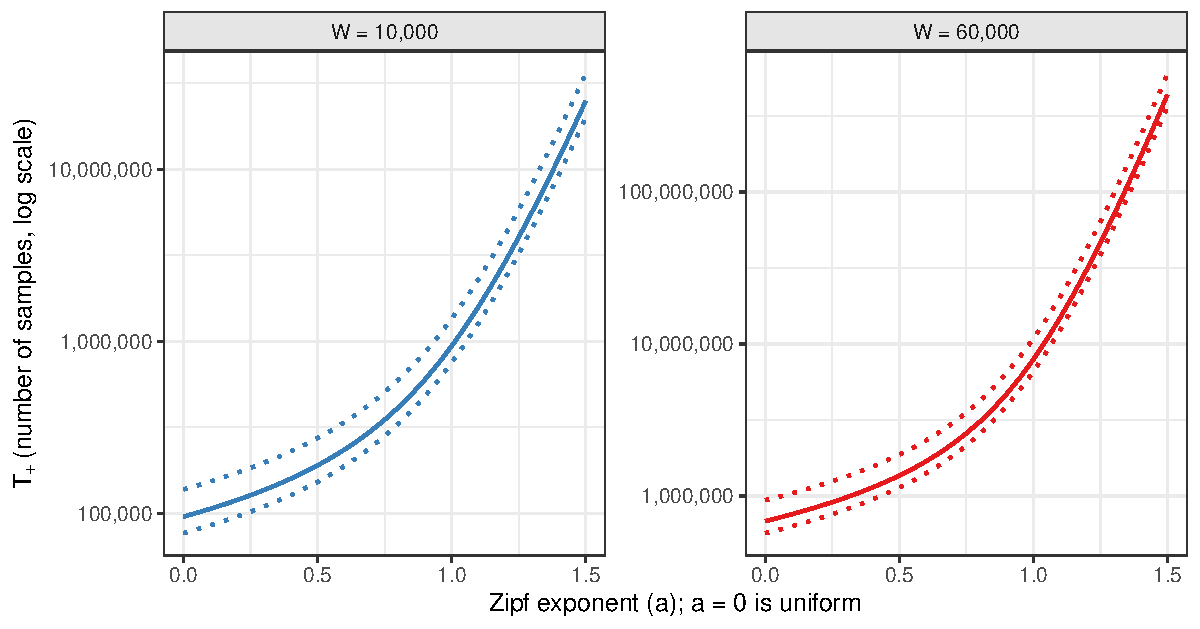
\includegraphics[width=\linewidth]{fig_estimate_R.pdf}
\caption{\label{fig-estimate} 
The required number of samples ($M$) from a generalized Zipf distribution ($p_{k} = k^{-a}/\sum_{k=1}^{N}k^{-a}$) needed for 1\%, 50\%, and 99\% of learners ($\epsilon$ = [.99, .01]; dotted lines, $\epsilon$ = 0.5; solid line) to reach a vocabulary size of $N = 10000$ or $N = 60000$, for varying values of the distribution exponent $a = 0, \ldots, 1.5$. A value of $a = 0$ corresponds to a uniform distribution. The number of samples is numerically calculated by the root of Equation (\ref{eqA-M}) in Appendix 1.} % what's the empirical a for CHILDES? ~1.5?
\label{fig}
\end{center}
\end{figure}

\subsection{Empirical dataset} % Shohei, maybe we should just refer to your other paper's estimate of the CHILDES exponent?
Given these theoretical implications, we analyze an empirical WF distribution of child-directed speech in the CHILDES corpus \citep{MacWhinney1990}--itself part of a broader pattern, since child-directed speech has recently been shown to be Zipfian across fifteen languages from seven language families, from six months of age onward \citep{LaviRotbain:2023}.
Figure~\ref{fig-freq} shows the word distribution from a CHILDES word-frequency export, from which we exclude hapax legomena (words occurring exactly once)--the words most likely to be idiosyncratic to a single household (e.g., a pet's or sibling's name) rather than genuinely rare in any individual child's actual input--leaving 27,673 words.
The minimal word probability was $2.616 \times 10^{-7}$, which gives the upper bound $T_{+} = f_{27673, 0.01}(2.616 \times 10^{-7}) = 5.669 \times 10^{7}$
or the median estimate $T_{+} = f_{27673, 0.5}(2.616 \times 10^{-7}) = 4.050 \times 10^{7}$. These estimates of required samples, being an order of magnitude larger than the optimistic theoretical estimate, suggest that this empirical Zipfian WF distribution would be difficult to learn.

A caveat about this estimate is worth making explicit, since Equation~(\ref{eq-Tbound})'s bound $T_{+}$ is driven entirely by the single least-frequent word in the corpus, and excluding hapax legomena only partially addresses the concern that rare words in a finite, pooled corpus may not reflect any individual child's actual input.
Removing all words rarer than 11 occurrences in the corpus (a considerably more aggressive filter, leaving 10,179 words) shrinks $T_{+}$ further, to $9.52\times10^{6}$, which is close to the analytical, idealized-Zipfian estimate from earlier in this section.
Working in the opposite direction, a corpus of this size may also under-sample genuinely rare but widely-shared words, pulling the estimated minimum probability--and hence $T_{+}$--the other way.
Because we cannot fully adjudicate between these two sources of bias without frequency counts drawn from individual children's longitudinal input rather than pooled across families, and because the qualitative conclusion is unchanged across all three filtering choices (only the precise magnitude moves, within a single order of magnitude), we treat the CHILDES-based estimate reported here as illustrating the same order-of-magnitude difficulty implied by our idealized Zipfian analysis above, rather than as a precise quantitative bound in its own right.

As an independent check on this concern, we repeated the calculation using a large word-frequency list derived from the Google Books corpus \citep{Michel:2011}, an entirely different source (adult written text rather than child-directed speech) with no relationship to CHILDES's transcript-pooling procedure. This list contains 97,565 words, but--critically for our purposes--only those with a raw corpus count of at least 100,000, i.e., it is truncated well short of the true long tail of rare words. Even so, its least-frequent entries give a minimal word probability of $1.344\times 10^{-7}$, yielding $T_{+} = f_{97565,0.01}(1.344\times 10^{-7}) = 1.197\times10^{8}$--within the same order of magnitude as the CHILDES-based estimate above, despite the two corpora differing enormously in size, genre, register, and collection method. Because this list's truncation necessarily omits rarer words than the ones it reports, $1.197\times10^{8}$ should if anything \textit{understate} the true $T_{+}$ for the full Google Books distribution, making this comparison a conservative cross-check rather than an inflated one. The convergence of two very differently-constructed corpora on the same order of magnitude is reassuring: it suggests the CHILDES-based conclusion is not an artifact of that corpus's particular size or composition.
%% See also test_fastmap.m in the XSL folder for more detail.

\begin{figure}[h]
\begin{center}
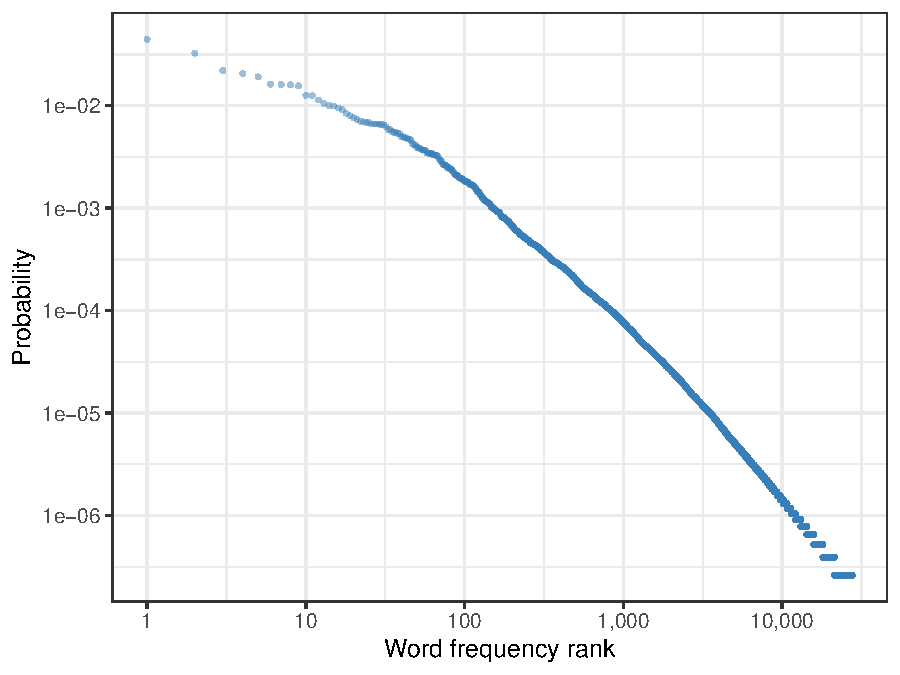
\includegraphics[width=\linewidth]{fig_freq_R.pdf} % width=9cm
\caption{Word frequency (rank vs.\ probability, log-log) in a CHILDES child-directed speech export, excluding hapax legomena (27,673 words).}
\label{fig-freq}
\end{center}
\end{figure}

%% Shohei added this section on Nov 9th, 2016.
\section{Active learning: Choosing situations}
\label{sec-active}
\subsection{Formulation}
The mathematical analysis above suggests that even the power of fast-mapping may not be efficient enough to learn Zipfian WFDs, raising the question of what mechanisms enable children to learn the nonuniform distributions they experience.
We explore one way to reconcile this discrepancy by adjusting the assumption about how about meanings are sampled in each situation.
In the analysis so far, the learner is assumed to be {\it passive}, having no choice but to observe and learn from a given situation: a randomly-sampled set of of objects, of which a (random) subset are labeled with words. 
The simplifying assumption of a passive learner likely underestimates real learners (and caregivers), who have some control over which situations are experienced.
Here, we consider a type of active learner who is able to {\it actively} choose the situations from which she learns words.
Returning to the toy example from the Methods section: rather than being handed a random toy, an active learner (or their caregiver) can choose to set up a particular scene--say, gathering the ball, the car, and the hat, rather than the ball, the cup, and the dog--and different scenes make different words more or less likely to be spoken by a caregiver.

Suppose that there are $N$ word-referent pairs and $M$ possible situations (e.g., scenes the learner could construct), and that the conditional probability to observe the $i^{\text{th}}$ word-referent pair is $p_{ij}$ given the $j^{\text{th}}$ situation.
Assume the active learner can choose the next learning situation from the given $M$ situations. %from which she learns the word-referent pairs.
Suppose that the active learner chooses the $j^{\text{th}}$ situation with probability $q_{j}$.
Denote the $N \times M$ matrix of conditional probabilities by $P = \{ p_{ij} \}_{ij}$ and the $N \times 1$ vector of the situation choice probabilities by $q = (q_{1}, q_{2}, \ldots, q_{M})^{T}$.
Thus, the marginal probability of word-referent pairs is given by the vector $Pq \in \mathbb{R}^{N}$.
Concretely, if the learner always constructed the same scene $j$, the words they would hear would simply follow that scene's column of $P$; by mixing across scenes according to $q$, the learner reshapes the overall word frequency distribution they experience, $Pq$, relative to whatever distribution a passive observer of randomly-constructed scenes would encounter.
According to the analysis in the previous section, the minimal probability of referents (or words) determines the number of samples required to complete the word learning, meaning
the best choice for the active learner is given by the choice probability \footnote{In the context of game theory, this optimal $\hat{q}$ corresponds to the max-min strategy (or Nash equilibrium) for the two-player zero-sum game defined by the payoff matrix $P$ (see for instance \cite{Maschler:2013}). }
\[
 \hat{q} = {\arg\max}_{q} \min(Pq).
\]
In words, $\hat q$ is whatever mixture of situations makes the \textit{least}-likely word-referent pair as likely as possible--maximizing the minimum entry of $Pq$--because it is exactly this minimum probability that, as shown in the Independent fast-mapping learning section, determines how long the learner must wait to complete the vocabulary. Framed this way, active learning as formalized here does not change how quickly any individual word is learned once encountered; rather, it reshapes which words the learner is likely to encounter in the first place, spreading exposure more evenly across the vocabulary than random sampling of situations would.
This minimal probability, $\min(P\hat{q})$, gives the theoretical upper bound for the minimal number of samples $$T_{+}=f_{W,\epsilon}( \min(P \hat{q}) ).$$
This is an upper bound with the known $P$, because the probability matrix
$P$ is not known before empirical learning, and the active leaner also needs to estimate $P$ from the sample.

For a given matrix $P$, the optimal $\hat{q}$ can be computed by the iterated linear programming algorithm (see Appendix 3 for details). % algorithmic complexity of this? Iris van Rooij and Johan Kwisthout would care

As a baseline for the passive learner, we consider the average $\min( Pq )$ with the uniform distribution over the vector $q$--i.e., a learner (or caregiver) who constructs scenes without regard to which words the learner has already mapped to a referent, the counterpart of the randomly-sampled situations analyzed in the previous section, now expressed in terms of situations rather than words directly. This baseline's lower bound is given by Jensen's inequality $$\int_{q\in \Simplex{N}}\min( Pq ) (N-1)!\dd q \ge \min( P \one{N}/N ),$$
where the integral is taken over the $N-1$ dimensional unit simplex $q\in \Simplex{N}$.
For a sufficiently small $x \ll 1$ and $y \ll 1$, $f_{W,\epsilon}(x)/ f_{W,\epsilon}(y) \approx y/ x$.
Thus, the rate $$R = \min(P \hat{q})/ \min(P \one{N}/N)$$ gives a good estimate for the rate of efficiency, by which
active learning with the optimal probability $\hat{q}$ is $R$ times faster on average
than passive learning with a uniformly-randomly chosen probability vector $q$. % transition sentence explaining what we do

\subsection{Empirical evaluation}
% from Takuma's presentation: 131067 Images, 908 Scene categories, 313884 Segmented objects, 4479 Object categories
To evaluate the potential impact of active leaning, we study the SUN database \cite{SUN2010} as an empirical estimate of object distributions in a collection of real-life scenes, reconstructing the $N \times M$ conditional probability matrix $P$ directly from the raw per-image object annotations (25,294 images), with each column normalized to give the conditional probability of each object given a scene category.
This reconstruction reproduces $N = 3,458$ objects and $M = 1,111$ scene categories exactly, and recovers the $\min(Pq)$ and $\min(P\hat q)$ values reported below to four significant figures, giving us confidence that it faithfully reconstructs the original analysis.
With uniform scene choice probability $q = \one{M}/M$, the $\min(Pq)$ is $8.30\times 10^{-9}$.
Meanwhile, with the optimal $\hat{q}$, the $\min(P\hat{q})$ is $1.95\times 10^{-6}$, indicating active learning is approximately $R = 235.3$ times faster than the baseline passive learning.
The marginal probability distributions of objects for the baseline and optimal $q$ are shown in Figure \ref{fig-optimalQ}.
The difference between the two marginal distributions is visible at their tails: the tail of the uniform $q$ decreases like an exponential function, but that of the optimal $\hat{q}$ decreases as a power function (linear in the log-log plot).

Having access to the underlying data lets us answer directly, rather than by conjecture, a question raised in an earlier version of this analysis: is the passive marginal realized under uniform scene selection more or less severe than the idealized Zipfian distributions analyzed in the Independent fast-mapping learning section?
Treating the $N=3,458$ objects as a vocabulary and applying Equation~(\ref{eq-Tbound}) directly to this real marginal gives $T_{+} = f_{3458,0.01}(8.30\times10^{-9}) \approx 1.54\times10^{9}$ episodes for the passive baseline, and $T_{+} = f_{3458,0.01}(1.95\times10^{-6}) \approx 6.52\times10^{6}$ episodes for the optimal active learner.
For comparison, a standard idealized Zipfian distribution ($a=1$) over the same $N=3,458$ items would require only $T_{+}\approx 3.85\times10^{5}$ episodes under passive fast-mapping--meaning the real, empirically-derived passive object distribution is roughly {\bf 3,990 times harder} to learn from than an idealized Zipfian of the same size, not easier, as we had speculated before this underlying SUN data could be located.
If anything, then, the $235\times$ active-learning speedup we report here likely {\it understates} the benefit active learning would confer relative to the idealized Zipfian baseline used elsewhere in this paper: real-world object distributions realized by unstructured (uniform) scene sampling appear to be considerably more extreme than the textbook Zipfian case, which if anything strengthens the case for active structuring of learning situations.
This empirical evaluation suggests that this form of active learning can make fast-mapping orders of magnitude more efficient.

\begin{figure}[h]
\begin{center}
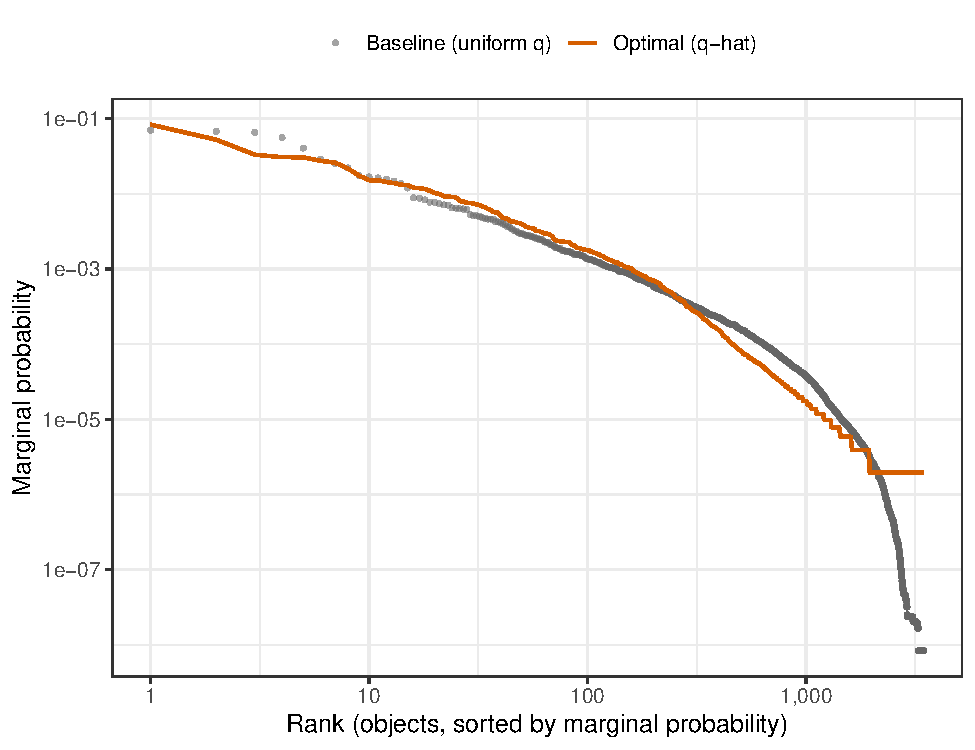
\includegraphics[width=\linewidth]{fig_optimalQ_R.pdf}
\caption{The marginal probability of referents for the optimal $\hat{q}$ (line) and its baseline (dots).}
\label{fig-optimalQ}
\end{center}
\end{figure}

\subsection{Online active learning with an unknown $P$}
%\todo[inline, color=green!40]{As Reviewer 3 misunderstand this and previous section, Shohei would clarify these sections.}
The above measure of active learning's efficiency is based on the optimal $\hat{q}$ with full knowledge of $P$, which gives an optimistic estimate of learning time since the matrix $P$ is unlikely to be fully known to the learner. 
Thus, we perform a Monte Carlo simulation to quantify the efficiency of an {\it online} active leaner who gradually learns $P$ and estimates $q$ based on the sample estimate of $P$. 
If this online active leaner is comparable to the optimal active learner with $\hat{q}$, we can treat the performance analysis of the optimal active leaner above (a few orders more efficient) as holding for the online active leaner. 
For this purpose, we generated a $N \times M$ matrix $P$ with $N=1000, M=100$, which has the elements in each column are Zipfian probabilities $P_{\pi(i)} \propto i^{-a}$ with random coefficients $a \in [1, 1.5]$, where $\pi: \{1, \ldots, N\} \mapsto \{1, \ldots, N\}$ is a random permutation. 
The online active learner has uniform choice probability $q_{1} = \one{N}/N$. 
For $k^{\text{th}}$ batch of 1000 steps, the online learner samples the objects according to the probability $P q_{k}$, and constructs the sample probability matrix $\hat{P}_{k}$ according to sample frequency. 
After the $k^{\text{th}}$ sampling step, the online learner estimates $q_{k} := \argmax_{q} \min( \hat{P}_{k} q )$. 
In each run of this procedure, we repeat up to $100 \times 1000$ samples, and obtain one sample for the number of required samples to finish learning names for all of the 1000 referents--the approximate vocabulary size of a 3-year-old. 

With 100 runs, we obtain the Monte Carlo estimate of the online learner shown in Figure \ref{fig-online}.
Figure~\ref{fig-online} shows the sample probability distribution of the number of required samples in the Monte Carlo simulation (circles: histogram, line: smoothed estimate), and its comparable median estimate for the optimal learner (green vertical line) and the passive learner with the uniform $q$ (red vertical line).
This simulation result shows that the online learner is, on average, as fast as an optimal learner, and is almost always faster than the passive learner, which requires twice as many samples.

Beyond the case study reported above, we also provide a theoretical analysis of why such online learning is possible in Appendix 4.

\begin{figure}[h]
\begin{center}
%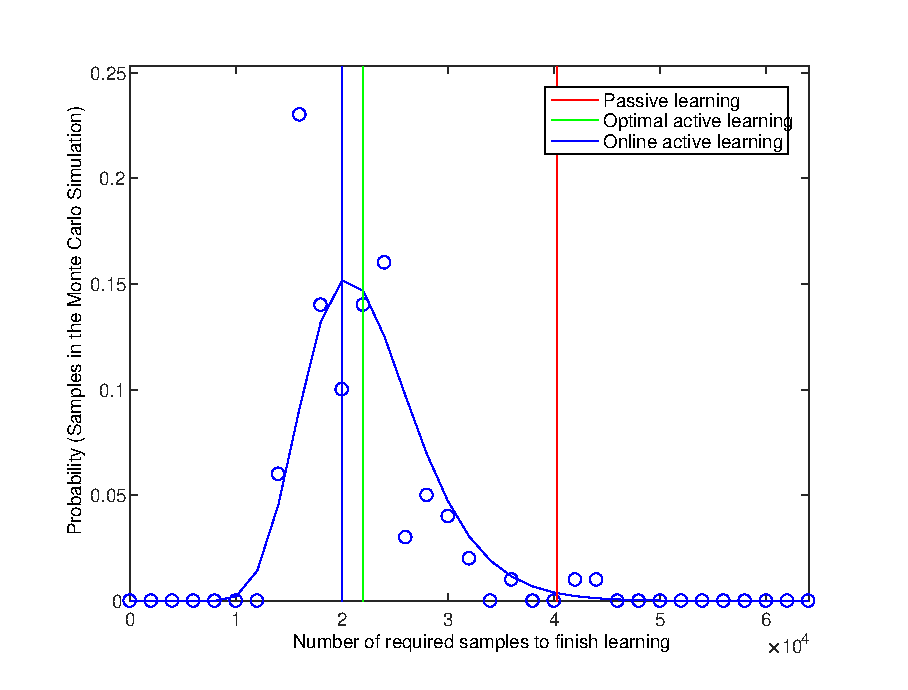
\includegraphics[width=9cm]{OnlineActiveLearning.eps}
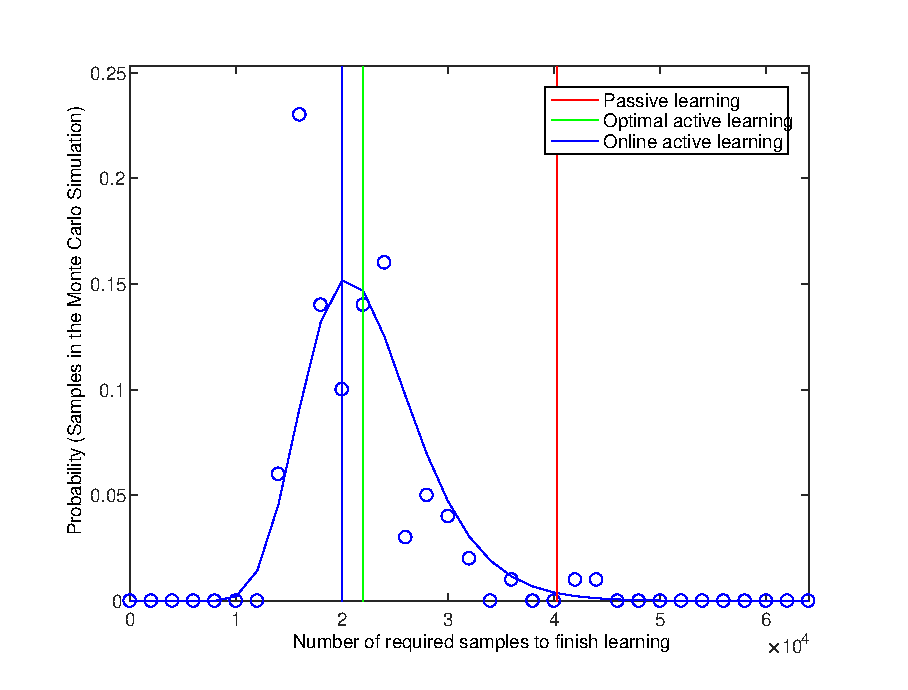
\includegraphics[width=\linewidth]{OnlineActiveLearning.eps}
\caption{The probability distribution of the number of required samples to finish learning for passive (red), optimal (green), and online active learners (blue). On average, online active learning was as fast as optimal active learning.}
\label{fig-online}
\end{center}
\end{figure}

\section{Incremental active learning}
\label{sec-incremental-sim}

The analyses above--both the fast-mapping bound of the Independent fast-mapping learning section and the idealized and online active learners of the Active learning section--all assume that a word is learned the moment it co-occurs with its target referent. This lets us derive clean analytical results, but it sidesteps a concern raised about this modeling tradition more broadly: that conclusions about learning speed may reflect the {\it sampling} process (how often the right word-referent pair happens to co-occur) rather than anything about {\it learning} itself, since treating learning as instantaneous leaves no room for the two to be distinguished. To test whether our qualitative conclusions--that passive sampling from a Zipfian distribution is implausibly slow, and that active learners can close much of this gap--survive when this instantaneous-learning idealization is relaxed, we simulated a learner who accumulates evidence across multiple exposures rather than fast-mapping. This simulation leaves a second idealization untouched: as in all the models in this paper, words are still learned fully independently of one another, with no transfer of information from an already-learned word (e.g., ``dog'') to a related but distinct one (e.g., ``cat''). We return to this remaining simplification, and its likely direction of bias, in the Discussion.

\subsection{Two incremental learning mechanisms}
We implemented two learners that both require multiple exposures to learn a word--unlike fast-mapping--but that differ in how they use those exposures, letting us ask whether our conclusions are a property of incremental learning in general or an artifact of one particular mechanism.

The first, an {\it eliminative} learner following \cite{Vogt:2012} and \cite{Siskind:1996}, tracks, for each word, the full set of referents it remains consistent with across all past exposures. In each episode, the learner observes a target word alongside $C-1$ distractor referents (as in the Active learning section); rather than immediately committing to a mapping, the learner eliminates from the word's candidate set any referent that was absent from the current situation. A word is considered learned once its candidate set has been narrowed to a single referent--i.e., once enough situations have ruled out every other possibility.

The second, a {\it guess-test} learner in the spirit of the propose-and-verify hypothesis-testing models discussed in the Introduction \citep[e.g.,][]{Trueswell:2013}, tracks only a single current best guess per word rather than a full candidate set. A word with no guess proposes one: an "unclaimed" referent from the current situation not already guessed by some other word. A held guess is discarded--forcing a new proposal next time--if a later exposure to that word does not include it, since the true referent is always present whenever its word is spoken (an assumption standard throughout this modeling tradition, and one that turns out not to be load-bearing: \cite{Blythe:2016} show that cross-situational learning still succeeds in the long run even when the target meaning is not always inferred, provided it remains the most frequently inferred candidate over time), so a guess that goes missing must be wrong. A word counts as learned once its current guess matches its true referent and has not since been discarded. This is a cheaper mechanism than full elimination (tracking one hypothesis instead of an entire candidate set), and, because a word's fate now depends on competition with other words for the same unclaimed referents, it can make genuine errors that later need correcting, rather than only ever narrowing monotonically toward the truth.

Both are strictly harder learning problems than fast-mapping: a single co-occurrence is no longer sufficient, and how quickly a word is learned depends on {\it which} distractors happen to accompany it, not only on how often it is sampled.

We crossed this incremental learner with the same two dimensions of active control introduced above, but now made concrete for both the target word and the distractors that accompany it, following the toy example from the Methods section:
\begin{itemize}
\item {\bf Target selection}: a \textit{passive} learner encounters a target word/referent sampled according to the (uniform or Zipfian) word frequency distribution; an \textit{active} learner instead preferentially selects situations built around a referent whose word is not yet known (e.g., choosing to play with the car rather than the already-learned ball).
\item {\bf Distractor (context) selection}: under \textit{random} context selection, the $C-1$ distractors accompanying the target are drawn according to the word frequency distribution, as in the Independent fast-mapping learning section; under \textit{familiar} context selection, distractors are drawn preferentially from referents whose candidate sets have already been narrowed down (i.e., toys the learner already knows a great deal about), which should make it easier to eliminate them as competitors for the target's word. This mechanism formalizes a disambiguation strategy with direct developmental support: children as young as two systematically exclude already-known objects as candidate referents for a novel word, and do so more reliably the better they already know those objects \citep{Grassmann:2015}--precisely the informal mutual-exclusivity intuition our elimination rule implements. It is also consistent with computational and observational evidence that non-co-occurrence information--including which referents have recently been discussed or attended to, and not just which are visually present--measurably improves reference resolution in cross-situational word learning \citep{FrankGoodmanTenenbaum:2009,FrankTenenbaumFernald:2013}.
\end{itemize}
This $2\times2$ design (active/passive target selection $\times$ random/familiar context selection), crossed with uniform and Zipfian word frequency distributions, lets us ask which forms of active control matter, and whether their benefits depend on the frequency distribution being learned--all without assuming fast-mapping.

\subsection{Simulation design}
We simulated vocabularies of $M = 1000$ referents--comparable to a 3-year-old's productive vocabulary, and consistent with the pre-literacy scope discussed in the Introduction--with Zipfian word frequencies $p_r \propto r^{-a}$ over frequency rank $r$, matching the exponent parametrization of the Independent fast-mapping learning section so that results are directly comparable to Figure~\ref{fig-estimate}. We crossed both learning mechanisms (eliminative, guess-test) with target selection (active/passive), context selection (random/familiar), and word frequency distribution (uniform; Zipfian with $a \in \{0.5, 1, 1.5\}$), at two context sizes, $C=10$ and $C=100$, chosen to fall on either side of \cite{Vogt:2012}'s reported $C/M \le 0.1$ tractability boundary ($C/M = 0.01$ and $0.1$ respectively at $M=1000$). We ran 30 replications per cell and recorded the number of episodes needed to learn 99\% of the vocabulary.

Two cells were computationally intractable to brute-force within a reasonable budget and are noted as such where relevant: the eliminative learner's cost scales with $M$ regardless of $C$ or exponent (it maintains a full $M$-length candidate set per word), and passive, randomly-sampled learning at $C=100$ under a steep Zipfian distribution ($a \ge 1$) requires both very many episodes and expensive per-episode bookkeeping--a single replication did not complete in 42 minutes. We report these cells using the already-validated analytical bound (Equation~\ref{eq-Tbound}) or, where real prior simulation data existed from earlier stages of this project (using a different but comparable Zipfian parametrization), that data, rather than a fresh, possibly-biased partial simulation. We also do not report an $M=10{,}000$ extension of this design (which we attempted, motivated by the pre-literacy vocabulary target discussed in the Introduction): even active-target conditions at this scale proved unpredictably expensive for the eliminative learner, and we judged further compute expenditure not to be a good use of the resources available for this project. The guess-test learner's cost does not scale with $M$ in the same way and was tractable throughout.\footnote{Simulation code, raw results, and the original (superseded) $M=1000$--$2000$ simulation results referenced in an earlier version of this analysis are available in the project repository (\texttt{corpusXSL/analysis/learners.R}, \texttt{corpusXSL\_eliminative\_active\_parallel.R}).}

\subsection{Results: context size interacts with active control}
Table~\ref{tab-incremental} and Figure~\ref{fig-incremental-sim} summarize the eliminative learner's mean episodes to learn 99\% of a $M=1000$-word Zipfian ($a=1$) vocabulary, at $C=10$ and $C=100$.\footnote{The $C=100$ passive/random cell used prior simulation data under a comparable but not identical Zipfian parametrization (Zipf-Mandelbrot, $p_r \propto (r+2.7)^{-1}$), as noted in the Simulation design; all other cells use the general $p_r \propto r^{-a}$ form.} Two things stand out. First, replicating our earlier conclusion, passive random sampling is dramatically slower under a Zipfian than a uniform distribution at both context sizes, and active target and context selection both help. Second, and not previously appreciated, {\it how much} each form of active control helps depends sharply on $C$, in a way that connects directly to \cite{Vogt:2012}'s observation that learning time depends on the ratio $C/M$: at $C=10$ ($C/M=0.01$, well inside Vogt's tractable range), familiar-context selection provides only a modest additional benefit on top of active target selection (2.0x alone, 28.6x combined with active targeting), because elimination is already fairly effective when the distractor set is small. At $C=100$ ($C/M=0.1$, right at Vogt's reported boundary of tractability), familiar-context selection becomes the dominant lever: alone it provides a 144.6x speedup, and combined with active target selection, a 1,292x speedup--because once $C$ is large enough that elimination from random distractors is itself close to intractable, ensuring that most of the $C-1$ distractors are already-resolved (and thus non-competing) referents is what actually rescues learning, more so than controlling which word is targeted.

\begin{table}[h]
\centering
\caption{\label{tab-incremental} Mean episodes to learn 99\% of a Zipfian ($a=1$), $M=1000$-word vocabulary, eliminative learner. Speedup is relative to Passive/Random at the same $C$.}
\begin{tabular}{lrrrr}
\hline
 & \multicolumn{2}{c}{$C=10$ ($C/M=0.01$)} & \multicolumn{2}{c}{$C=100$ ($C/M=0.1$)} \\
Condition & Episodes & Speedup & Episodes & Speedup \\
\hline
Passive / Random    & 89{,}454    & 1x      & 11{,}751{,}913 & 1x \\
Active / Random     & 4{,}695     & 19.1x   & 713{,}244      & 16.5x \\
Passive / Familiar  & 44{,}607    & 2.0x    & 81{,}269       & 144.6x \\
Active / Familiar   & 3{,}127     & 28.6x   & 9{,}093        & 1{,}292x \\
\hline
\end{tabular}
\end{table}

\begin{figure}[h]
\begin{center}
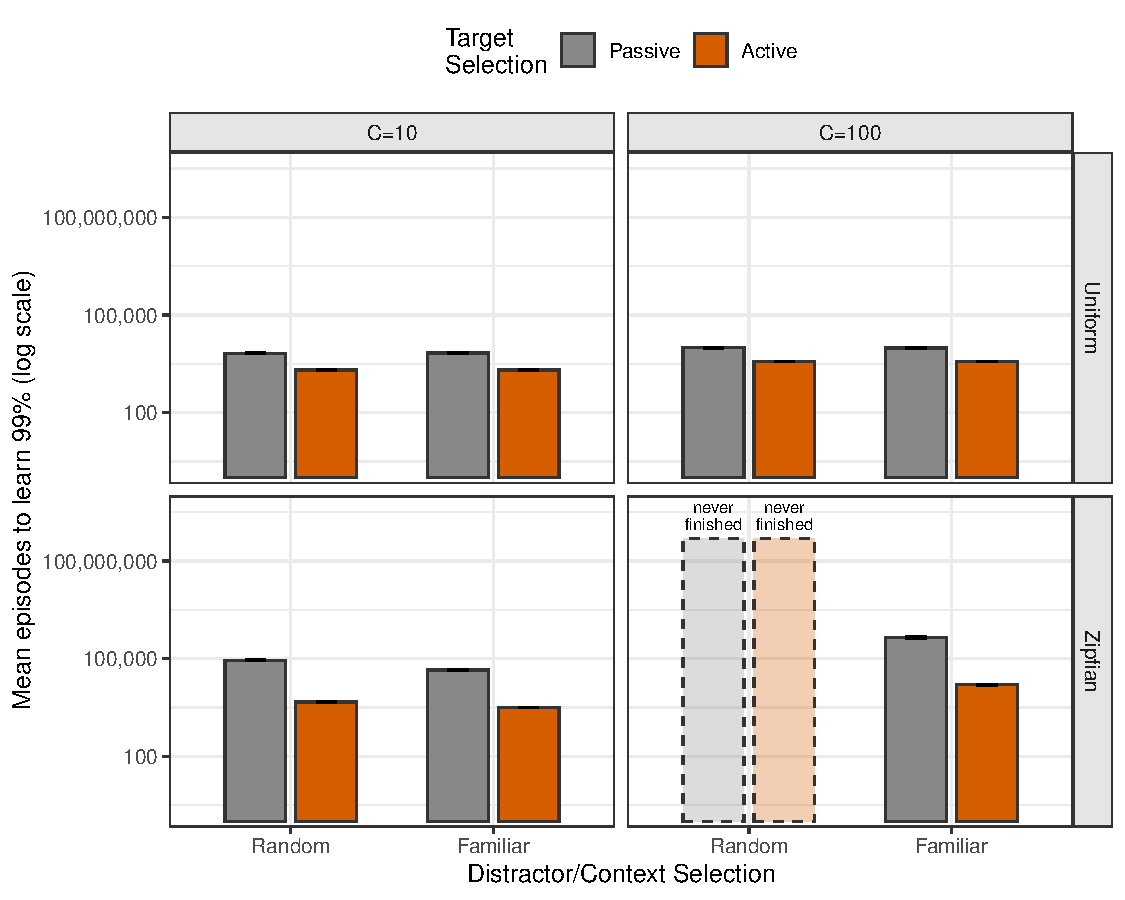
\includegraphics[width=\linewidth]{incremental_sim_summary.pdf}
\caption{\label{fig-incremental-sim}
Mean episodes (log scale, $\pm$ 1 SE) required for an incremental, elimination-based learner to acquire 99\% of a 1000-word vocabulary, as a function of whether the target word is sampled passively or actively selected to be unknown (bar fill), and whether distractors are drawn randomly or preferentially from familiar (already partly-known) referents (x-axis), separately for uniform and Zipfian word frequency distributions. Results are averaged over context sizes $C=10$ and $C=100$; see Table~\ref{tab-incremental} for the values disaggregated by $C$, which differ considerably.}
\end{center}
\end{figure}

These results reinforce the paper's central conclusions using a learner that makes neither of the two idealizations most often raised against fast-mapping models: words are not learned on a single exposure, and the number of samples required is not simply a proxy for how often a word is spoken. They also reveal that the two forms of active control we distinguish--choosing what to talk about, and choosing what else is nearby when talking about it--are not interchangeable, and that their relative importance is itself a function of how large the situation is relative to the vocabulary, echoing and extending \cite{Vogt:2012}'s $C/M$ finding to the active-learning setting.

The three subsections that follow subject this core result to further scrutiny, asking in turn whether it depends on reporting a single vocabulary-completion target, a single Zipf exponent and learning mechanism, or an idealized assumption about memory.

\subsection{How much of the vocabulary matters}
\label{sec-checkpoints}

The comparisons above, like most of this literature, summarize learning speed with a single number: episodes needed to reach 99\% of the vocabulary. This is a natural default--it mirrors how ``learned'' is operationalized throughout this paper, including the fast-mapping bound of the Independent fast-mapping learning section--but it is also, by construction, dominated by whichever handful of words are hardest to acquire, typically the rarest ones under a Zipfian distribution. Two questions follow. First, does reporting a mean conceal a badly skewed distribution, such that a ``typical'' simulated run looks nothing like the reported average? Second, and more substantively, is the size of the active-learning advantage we report specific to the choice of 99\% as a target, or does it hold at more modest completion targets?

To address both, we re-examined the same simulation data underlying Table~\ref{tab-incremental}, at three checkpoints--50\%, 90\%, and 99\% of the vocabulary known--rather than only the last. Each learner already records the episode at which every decile of the vocabulary is first reached, so this required no new simulation, only a finer-grained summary of data already collected.

On the first question, the answer is reassuring: mean and median are effectively indistinguishable at every checkpoint and condition we examined (ratio of mean to median between 0.99 and 1.02 throughout). Despite each individual word's own acquisition time being itself a highly skewed waiting-time process (see the Independent fast-mapping learning section), the total time to reach a given fraction of an $M$-word vocabulary averages over enough of these individually-skewed waits that the aggregate is close to symmetric. The means reported throughout this paper are therefore not artifacts of a long right tail; a typical simulated learner looks very much like the reported average.

On the second question, the completion target matters a great deal--not for whether active selection helps, but for how large the benefit appears to be. Table~\ref{tab-checkpoint} and Figure~\ref{fig-checkpoint} show the active/passive speedup at each checkpoint. In every condition, active selection is already a clear, non-trivial advantage at 50\% completion--a typical run through half the vocabulary is 1.7--4.1x faster under active selection. But the size of this advantage compounds sharply as the target moves toward completeness: it roughly doubles by 90\%, and doubles again by 99\%, reaching 19x for the eliminative learner at $C=10$. The single 99\%-only estimates reported elsewhere in this paper are therefore close to the maximum size the effect takes across this trajectory, not a representative one--informative in its own right, but not interchangeable with a claim about how much active selection typically matters for everyday word learning.

This bears directly on how Table~\ref{tab-incremental} and Figure~\ref{fig-incremental-sim} should be read. That the last one-in-a-hundred words of a Zipfian vocabulary take disproportionately, sometimes wildly, longer to acquire than the rest is a real and, we think, underappreciated property of frequency-driven word learning--but it is also the piece of these results most likely to reflect what this class of model leaves out, rather than how children actually learn the last few rare words of their lexicon. Real children have recourse to mechanisms with no analogue here--bootstrapping from already-known words, explicit correction, discourse and narrative redundancy, deliberate instruction--that plausibly matter most exactly where pure frequency-driven sampling is weakest: rescuing the rarest words from an otherwise very long wait. The best-supported claim from this analysis is therefore the more modest one: active selection provides a real, substantial speedup for reaching a \textit{functional} vocabulary, and Zipfian skew makes this advantage compound the more completeness is demanded of the learner--not that any specific number of episodes is required to reach a literal 99\% of an adult lexicon.

\begin{table}[h]
\centering
\caption{\label{tab-checkpoint} Active/passive speedup (ratio of mean episodes, passive over active; Zipfian, $a=1$, Random context) at three vocabulary-completion checkpoints. Median-based speedups (not shown) agree to within 2\% throughout. Guess-test at $C=100$ is omitted: per-checkpoint data were not preserved from that run (see the Simulation design above), though its 99\%-checkpoint speedup is reported above (Robustness across Zipf exponent and learning mechanism).}
\begin{tabular}{lrrr}
\hline
 & \multicolumn{3}{c}{Speedup at completion checkpoint} \\
Condition & 50\% & 90\% & 99\% \\
\hline
Eliminative, $C=10$  & 4.1x & 9.2x & 19.1x \\
Eliminative, $C=100$ & 3.1x & 7.5x & 16.5x \\
Guess-test, $C=10$   & 1.7x & 3.0x & 4.9x  \\
\hline
\end{tabular}
\end{table}

\begin{figure}[h]
\begin{center}
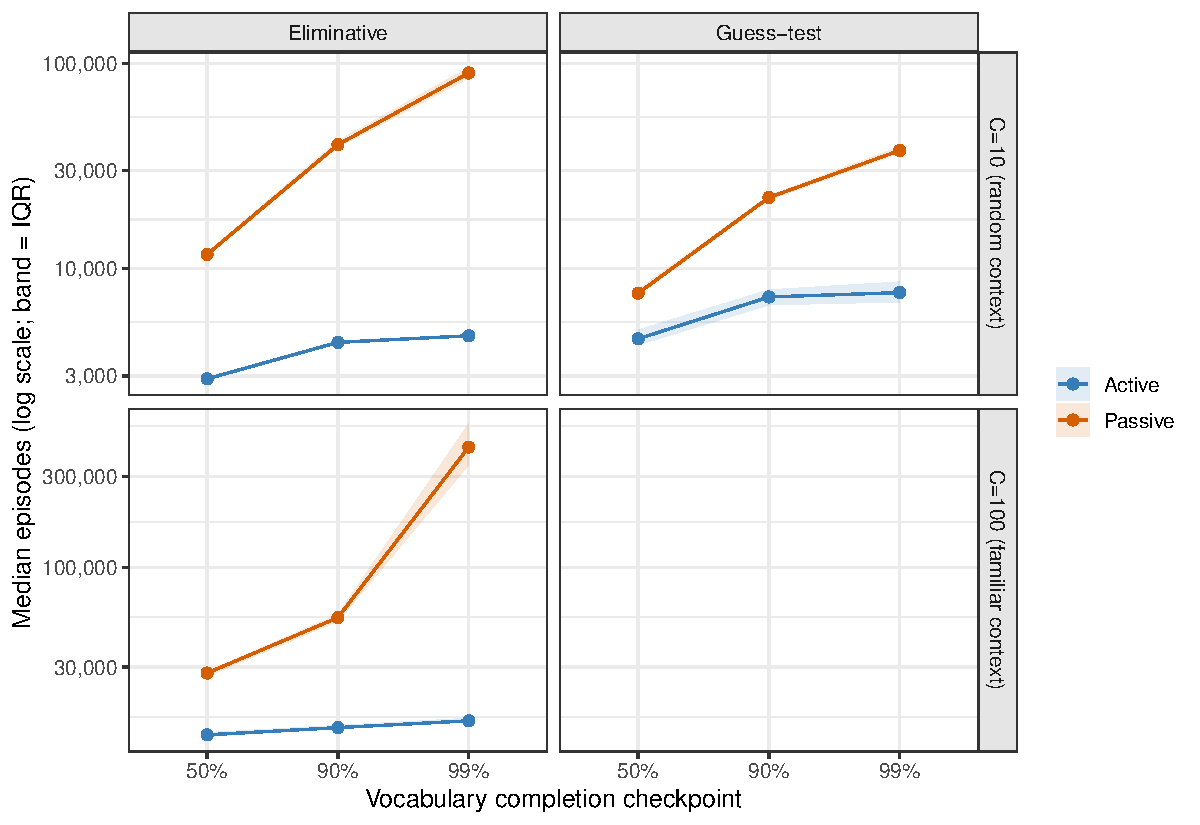
\includegraphics[width=0.8\linewidth]{checkpoint_divergence.pdf}
\caption{\label{fig-checkpoint}
Median episodes (log scale; band = interquartile range) to reach 50\%, 90\%, and 99\% of a Zipfian ($a=1$), $M=1000$-word vocabulary, active vs.\ passive target selection, by learning mechanism and context size. The active/passive gap widens steadily with the completion target rather than being a fixed multiplicative constant.}
\end{center}
\end{figure}

\subsection{Robustness across Zipf exponent and learning mechanism}
Two further checks address whether these conclusions are specific to $a=1$ or to the eliminative mechanism. First, varying the Zipf exponent at $C=10$ (Figure~\ref{fig-exponent}) shows the same dose-response pattern found analytically in the Independent fast-mapping learning section (Figure~\ref{fig-estimate}): passive learning slows super-exponentially as $a$ increases (eliminative passive/random: 6,676 episodes at $a=0$, 10,795 at $a=0.5$, 89,454 at $a=1$), and active selection's advantage grows accordingly.

Second, the guess-test learner shows the same qualitative pattern--Zipfian is harder than uniform, active selection helps, and the $C/M$ ratio matters--but with a substantially more modest magnitude, and one notable reversal. At $C=10$, $a=1$, guess-test's passive/random baseline (38,037 episodes) is already faster than the eliminative learner's, and active selection provides only a 4.9x speedup (vs.\ eliminative's 19.1x); familiar-context selection alone provides essentially no benefit (1.4x). At $C=100$, guess-test again shows more modest speedups than eliminative (roughly 2--4x across conditions, vs.\ eliminative's 16--1,292x), because its cost does not depend on $M$ the way full elimination does, and it is correspondingly less exposed to Vogt's $C/M$ bottleneck in the first place. Guess-test also handles steep skew ($a=1.5$) far better than eliminative does at $C=10$ (active/random: 37,570 episodes, vs.\ eliminative's 296,637--an 8-fold difference in the opposite direction from the $a=1$ comparison), since a single lucky unclaimed guess can succeed even when full elimination would require many more exposures to fully rule out a large, skewed distractor pool. Finally, at $C=100$, $a=1$, we found that combining active target selection with familiar-context selection produces a genuinely bimodal outcome for guess-test: most runs complete quickly (four of five diagnostic replications finished in 135,000--212,000 episodes), but a substantial minority become stuck in an extended standoff, apparently because familiarity-weighted distractor selection can concentrate the distractor pool onto a small set of already-claimed referents, starving the few remaining hard-to-place words of any unclaimed candidate to propose (one of five replications exceeded our three-million-episode computational budget without completing). This is a genuine, if unfortunate, emergent property of combining these two particular heuristics for this particular mechanism, and a reminder that not all combinations of otherwise-beneficial active strategies compose well.

Third, a \textit{ranked-frequency} learner--which tracks a full co-occurrence count matrix rather than a binary candidate set or a single guess, and counts a word as learned once its true referent has strictly the highest count among all candidates--shows real, Zipfian-sensitive passive slowdown at $C=10$ closely tracking the other two mechanisms (4,573 episodes at $a=0$; 6,754 at $a=0.5$; 22,777 at $a=1$), but revealed a more fundamental methodological lesson under active selection. Because this criterion counts a \textit{tie} for the maximum as success, and a word's very first exposure as an active target necessarily produces a tie (every referent that co-occurred with it, including its true referent, is incremented together from the same initial count), active target selection causes every word to register as learned on its first exposure--collapsing what should be a multi-exposure incremental learning process into an accidental restatement of fast-mapping. The result is not merely a smaller active-learning advantage, as with guess-test, but a degenerate one: episodes-to-99\%-learned under active selection is exactly $990$ (i.e., $M \times 0.99$) with zero variance across all 30 replications, at every exponent and both context-selection conditions, because active selection combined with this criterion guarantees exactly one newly-learned word per episode with no exceptions. We do not count this as evidence that active selection provides an unbounded benefit for this mechanism; rather, it reveals that a superficially reasonable ``was the true referent favored on the evidence so far'' criterion can be satisfied too easily when most of the count matrix is at its uninformative initial value, and is a caution about validating any single learning criterion's behavior under active selection specifically, not just under the passive conditions it may originally have been designed and tested against.

\begin{figure}[h]
\begin{center}
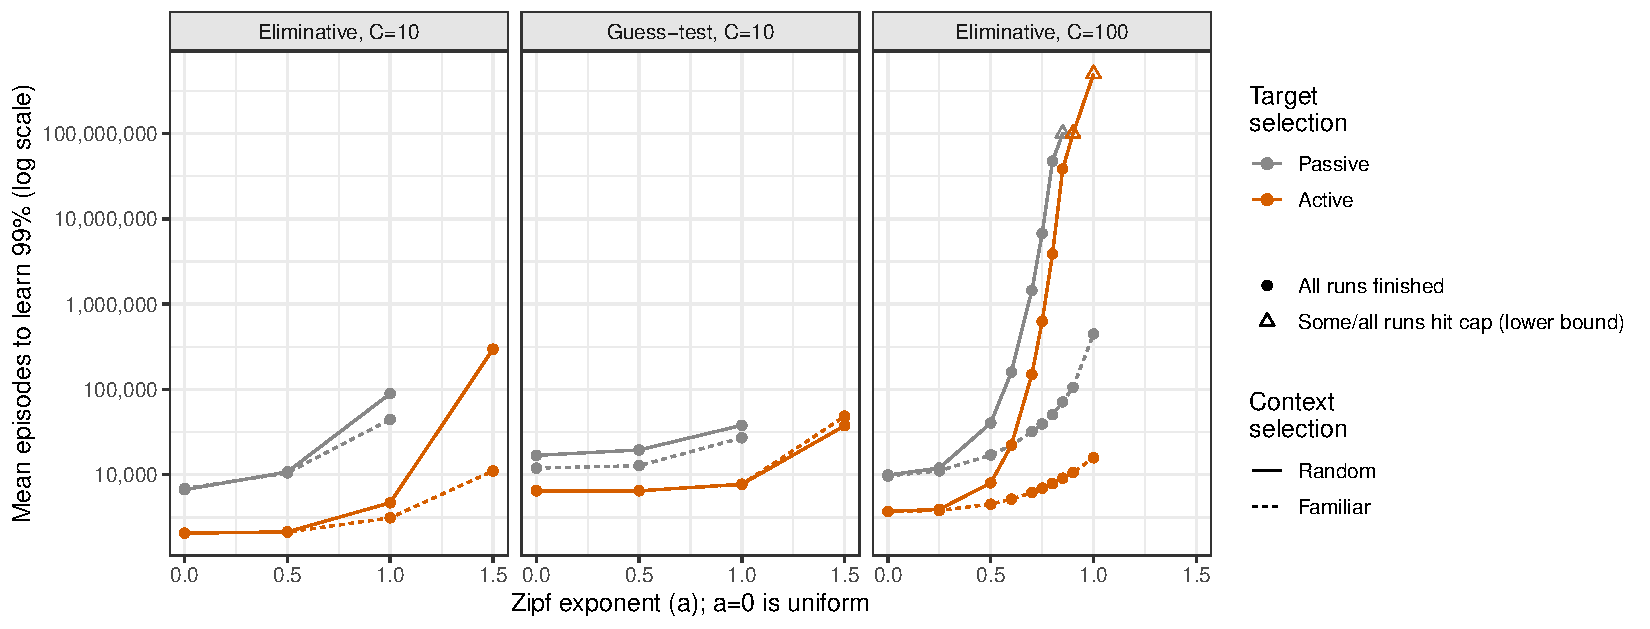
\includegraphics[width=\linewidth]{exponent_sensitivity.pdf}
\caption{\label{fig-exponent}
Mean episodes (log scale) for the eliminative learner to acquire 99\% of a 1000-word vocabulary as a function of the Zipf exponent $a$ ($a=0$ is uniform), separately by context size ($C=10$, $C=100$), target selection (color), and context selection (line type). Compare to the purely analytical, fast-mapping version of this dose-response relationship in Figure~\ref{fig-estimate}.}
\end{center}
\end{figure}

Together, these robustness checks support a more precise version of our central claim than the single-mechanism result alone would: active control over learning situations reliably helps under Zipfian sampling, and can help enormously, but the size of the benefit is not a fixed constant--it depends on the specific learning mechanism, the severity of the distributional skew, and, most surprisingly, on how large the local context is relative to the vocabulary being learned.

\subsection{Does the advantage survive forgetting?}
\label{sec-decay}

Every learning mechanism considered so far shares an idealization common to this modeling tradition: once evidence points toward a word-referent mapping, that evidence is retained indefinitely, with no possibility of a still-tentative guess simply being forgotten if it goes unrehearsed. This is a strong assumption, and one a skeptical reader might reasonably worry is doing unacknowledged work--if active selection's advantage partly reflects the model's own unlimited memory for guesses no real learner would retain that long, relaxing this idealization could narrow, or even reverse, the gap we report.

We tested this directly by adding a minimal forgetting mechanism to the guess-test learner (chosen because its propose-and-verify structure already tracks a natural target for decay: each word's current best guess). An unconfirmed guess--one not yet locked in as the word's final, correct mapping--now decays back to ``no guess'' with a constant per-episode hazard if the word goes unrehearsed; concretely, a guess survives $t$ episodes without its word being re-exposed with probability $(1-p)^t$, checked lazily only when the word is next targeted, so the mechanism adds no computational cost to episodes that do not involve it. A guess that has already resolved to the correct mapping--i.e., a word already counted as learned--is exempt: this is a claim about forgetting a tentative hypothesis, not about relearning already-acquired words, a different and more contentious claim we do not make here.

We predicted this manipulation would, if anything, widen rather than narrow the active-learning advantage. Active selection, by preferentially returning to whichever word it currently judges highest-priority among the unknown, incidentally functions as a rehearsal schedule: it revisits a word again long before a low forgetting hazard could plausibly erase its progress. Passive sampling has no such property--under Zipfian word frequencies, a rare word may go tens of thousands of episodes between successive exposures, giving a tentative guess ample time to decay before it can ever be reconfirmed or corrected.

The prediction was confirmed, and the effect was substantial and graded (Figure~\ref{fig-decay}). We calibrated the tested half-lives against the actual distribution of passive revisit gaps at $C=10$, $a=1$: the rarest word's expected gap between passive exposures is $\sim$7,485 episodes, and 97\% of words exceed a 200-episode gap, so we tested four half-lives spanning well below and above this range, $t_{1/2} \in \{20{,}000, 5{,}000, 1{,}000, 200\}$ episodes (equivalently $p \in \{0.000035, 0.000139, 0.000693, 0.003460\}$). The active condition stayed essentially flat across this entire range--6,963--8,166 episodes to learn 99\% of the vocabulary at every half-life tested, indistinguishable from the no-decay baseline of 7,656 regardless of how severe forgetting was made. The passive condition, by contrast, showed a clear dose-response gradient: 44,164 episodes at the longest half-life (barely above the no-decay baseline of 38,774, since a 20,000-episode half-life rarely bites before most words are revisited again) rising steadily to 52,186, then 64,068, then 69,880 episodes as the half-life shortened to 200. The active/passive speedup grew correspondingly, from 5.1x with no decay through 5.4x, 6.8x, and 9.2x, to 9.6x at the shortest half-life tested, and this pattern held at every completion checkpoint we examined (50\%, 90\%, and 99\%; see ``How much of the vocabulary matters,'' above), not only at the most demanding one. This gradient, rather than an abrupt jump from no effect to saturation, clarifies the mechanism: what matters for passive learning is specifically whether the forgetting half-life is short relative to how long a tentative guess must typically wait to be rehearsed, which under Zipfian sampling depends on how rare the word is. Active selection, by contrast, keeps its own revisit gaps short for whatever it currently prioritizes regardless of any word's rarity, so even the shortest half-life we tested could not make forgetting bite.

This result addresses a natural worry about this modeling tradition directly, rather than by argument: relaxing the idealization of perfect, unlimited memory for tentative hypotheses does not erode the case for active selection, because active selection's core mechanism--preferentially returning to what is not yet known--doubles as protection against exactly the kind of forgetting a more cognitively realistic learner would be subject to. If anything, this strengthens the paper's central claim: some of what active selection buys a learner may not be about sampling efficiency alone, but about how well a given sampling policy happens to align with the demands of a bounded, forgetting memory system.

\begin{figure}[h]
\begin{center}
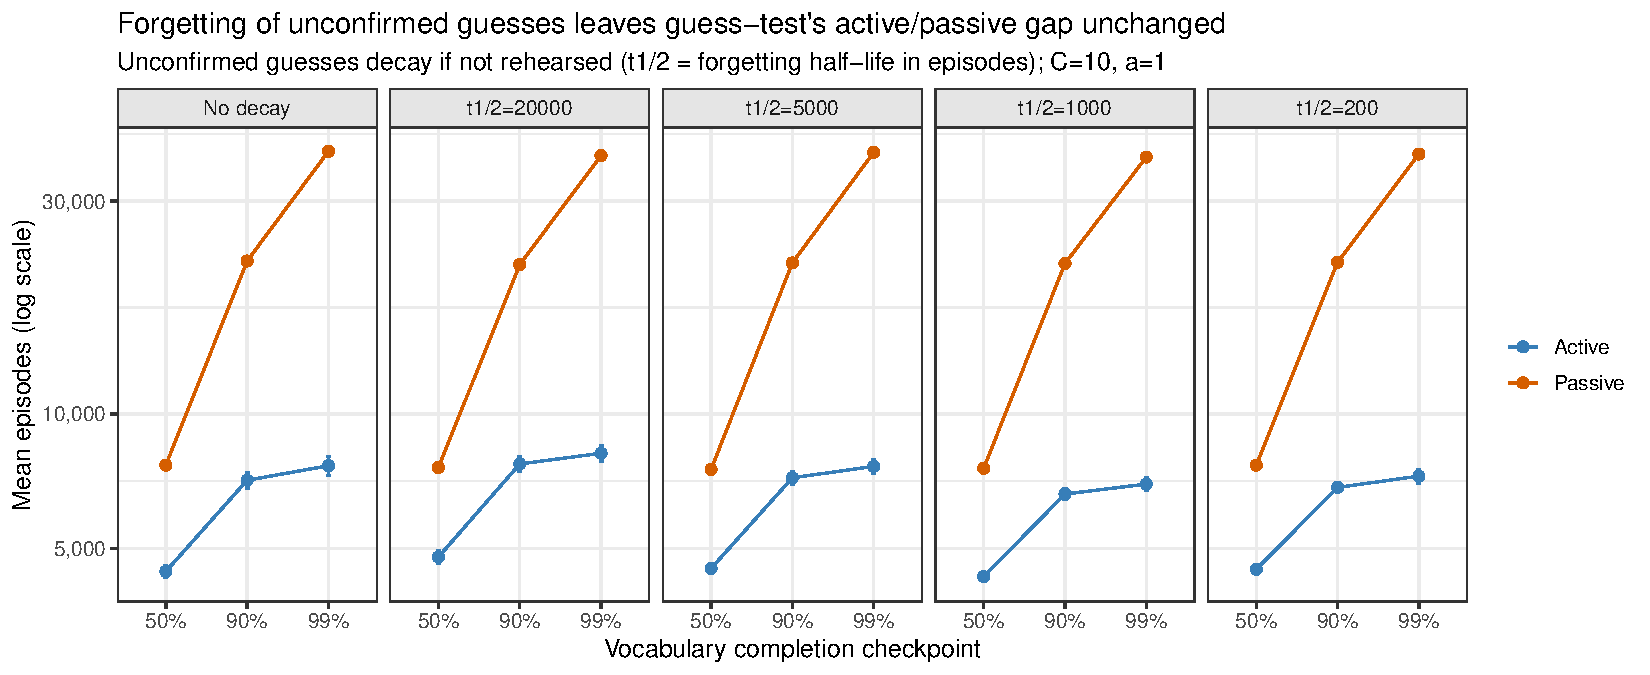
\includegraphics[width=\linewidth]{decay_sweep.pdf}
\caption{\label{fig-decay}
Mean episodes ($\pm$ 1 SE, log scale) for the guess-test learner to reach 50\%, 90\%, and 99\% vocabulary completion, active vs.\ passive target selection, at $C=10$, $a=1$, across five forgetting conditions (no decay, and forgetting half-lives of 20,000, 5,000, 1,000, and 200 episodes for an unconfirmed guess, chosen to span below and above the typical passive revisit gap). Forgetting leaves active selection essentially unaffected at every severity tested, while passive sampling slows along a clear dose-response gradient as the half-life shortens, widening rather than narrowing the active/passive gap.}
\end{center}
\end{figure}

\section{Discussion}

%This study offered a mathematical analysis of word learning, providing general constraints that any theoretical account of children's word learning should satisfy. 
This study reinspected the claim by \cite{Blythe:2010} that independently fast-mapping word meanings is efficient enough to learn a full adult lexicon in 18 years, extending the analysis to arbitrary (not only uniform or Zipfian) word frequency distributions, and complementing \cite{Vogt:2012}'s related but distinct analysis of Zipfian distractor sets under a different, elimination-based learning mechanism (see the Active learning section). % Vogt also suggested C - context size; incidental meanings - matters
Two further lines of related mathematical work address adjacent questions we do not, but are worth situating our contribution against. \cite{Blythe:2016} show that cross-situational learning remains tractable even under \textit{infinitely} many candidate meanings per word, provided their plausibility decays fast enough as they grow more implausible--a result that, structurally, mirrors our own central finding that a single extremal quantity governs learning time regardless of how large the surrounding space is (there, the most plausible confounder's decay rate; here, the least frequent word's sampling probability). \cite{Reisenauer:2013} show, for an elimination-based learner closely related to ours, that a mutual exclusivity constraint linking words together--rather than each word narrowing its candidates independently, as every learner in this paper does--can rescue learning from the same kind of super-exponential slowdown our own eliminative model exhibits at large $C$; we return to what this implies for our own numbers below.
We offer a first closed-form analytical bound on the learning time of an entire lexicon for an arbitrary word frequency distribution, consistent with the general intuition behind \cite{Vogt:2012}'s simulation results that learning time is governed by the probability of sampling the single least-frequent word.
Our new analysis showed that even fast-mapping--the most generous passive, independent learning scheme--implies an implausibly large number of samples for word distributions with a long tail of rarely-sampled words, including the Zipf distribution, and simulations of a more realistic incremental learner showed the same qualitative pattern (see the Incremental active learning section). % In essence, learners end up waiting a long time for the long tail of the distribution: low-frequency words are simply too rare.

% discuss relation to Hidaka2013 and MollicaPiantadosi2017 effective learning instances -- we define how ELIs might be constructed (for one-shot learners), while they estimate how -- constant factor (still reasonable amount of input?)
Given that our analysis implied learning would be too slow under realistic distributions, we considered a more efficient learning scheme, in which the learner can choose preferred learning situations by composing the contexts from which words are drawn. 
This type of active control over situations seems natural with respect to general observations of children's behavior \citep{Yu:2009active}, and has been shown to benefit adult word learners \citep{Kachergis:2013}, but has not to our knowledge previously been subjected to theoretical analysis. 
We quantify and evaluate the effect of this type of self-directed learning in word learning using a modeling framework with few assumptions \citep{Blythe:2010,Vogt:2012,Blythe:2016}. 
As the least probable word in the distribution determines learning efficiency, we analyzed the effect of active choice on the situations maximizing this key parameter. 
Analyzing an empirical dataset of labeled referents in a set of natural scenes, we found that the expected learning time of an idealized active learner--one with full advance knowledge of how referents co-occur with scenes, who still fast-maps each word--is over two hundred times (235x) more efficient than a passive learner sampling scenes uniformly at random; reconstructing this analysis from the underlying raw data (see the Active learning section) suggests this figure is, if anything, an underestimate of the true benefit relative to an idealized Zipfian baseline, since the real passive marginal turned out to be roughly 3,990 times harder to learn from than a standard Zipfian distribution of the same size.
Three further analyses show that this large speedup should nonetheless be treated as an upper bound on any single, representative estimate, both because the true advantage depends on several idealizations being relaxed together and because it varies with the specific learning mechanism assumed.
First, an active learner who must instead estimate this co-occurrence structure online from experience, rather than know it in advance, but who still fast-maps, requires only about half as many samples as its passive counterpart in our simulated setting (see the Active learning section)--a much smaller advantage than the idealized case, since the learner spends part of its budget discovering $P$ rather than exploiting it.
Second, a learner who cannot fast-map at all, but must instead accumulate evidence for word-referent mappings across multiple exposures, shows an advantage that depends heavily on context size: for an eliminative learner, active target selection alone yields a 16--19-fold advantage under a Zipfian distribution, and combining it with active control over the accompanying distractors yields a 29-fold advantage when contexts are small relative to the vocabulary ($C/M=0.01$), but a more than 1,000-fold advantage when contexts are large enough to approach \cite{Vogt:2012}'s reported tractability boundary ($C/M=0.1$; see the Incremental active learning section).
Third, this advantage is not a fixed property of ``incremental learning'' in general: a distinct propose-and-revise (guess-test) mechanism shows the same qualitative pattern but a substantially more modest magnitude (roughly 2--5x across conditions rather than 16--1,292x), because its cost does not scale with vocabulary size the way full elimination does, and is correspondingly less exposed to the $C/M$ bottleneck.
Taken together, these estimates span more than three orders of magnitude, from about 2x to nearly 4,000x, depending on which idealizations are relaxed: how much the learner already knows about its environment, whether learning requires one exposure or several, which specific learning mechanism is assumed, and how large the local context is relative to the vocabulary.
What remains stable across this range is the direction of the effect, not its exact size: some form of active control over learning situations reliably speeds up vocabulary acquisition under Zipfian word and referent distributions, and does so far more than under a uniform distribution, where active selection helps only modestly (see the Incremental active learning section).
Together, these results suggest that active choice in word learning is one plausible contributor to how children learn Zipfian vocabularies within realistic timeframes--not that passive learning plays no role, but that it is unlikely to be the whole story.
% We propose and analyze the learning time for a general active learning algorithm--including an online version.

This paper analyzed both an idealized fast-mapping learner and a more realistic incremental learner in order to characterize the effects of nonuniform word frequency distributions, with and without active learning.
\GK{We expect that other word learning mechanisms suffer to the same extent from nonuniform distributions in the environment, and future work can use the same analytic techniques presented here to confirm that.
Moreover, we expect that the active learning mechanisms presented are generalizable to other models, and will similarly alleviate the difficulty of learning from naturalistic nonuniform distributions.
Although the optimal active learning algorithm we have considered may not be cognitively plausible (and thus may predict faster learning than young children show), in conjunction with the fast-mapping mechanism it offers an upper-bound on the speed of active word learning, and future work should consider suboptimal active learning mechanisms that are more cognitively plausible.}
The cognitive plausibility of the specific mechanisms we simulate is a fair question to press on, and the evidence is genuinely mixed rather than uniformly supportive.
On one hand, infants preferentially attend to stimuli of intermediate, rather than minimal or maximal, predictability or complexity \citep[the ``Goldilocks effect'';][]{Kidd:2012}, consistent with our active learner's preference for referents whose words are not yet known but which are otherwise unremarkable; and self-directed, environment-adapted information search is documented in children from around age three onward \citep{Ruggeri:2022}, well within the age range relevant to our pre-literacy scope (see the Introduction).
On the other hand, at least one recent, well-controlled study found no advantage of active over passive information selection for infants' retention of novel word-object associations in a gaze-contingent paradigm \citep{Bazhydai:2026}, a direct empirical test of a claim close to the one we model computationally.
We do not think this null result undermines our central contribution--which is a computational characterization of how large an advantage active control {\it could} confer under Zipfian distributions, not a claim that children realize this advantage in full--but it is a reason for caution in treating our active-learning estimates as a description of typical development, rather than as an upper bound that motivates looking for partial, more constrained forms of active control. This caution is sharpened by our completion-checkpoint analysis (``How much of the vocabulary matters,'' above): the largest speedups we report are concentrated in the last stretch toward a fully complete vocabulary, a target more likely to reflect what our models leave out--mechanisms besides frequency-driven sampling that could plausibly rescue the rarest remaining words--than any real child's learning trajectory; the more modest, still substantial speedups evident already at 50--90\% completion are the better guide to what active selection buys a typical learner.
Our analysis also rests on simplifying assumptions common to this modeling tradition \citep{Blythe:2010,Vogt:2012,Blythe:2016} that are worth making explicit.
First, we assumed a mutually-exclusive lexicon in which each word maps to exactly one referent; in reality many words have synonyms, which may ease learning somewhat (evidence for one member of a synonym set can be informative about related words), but does not change our basic conclusion, since each synonym must still be individually sampled and learned under both the fast-mapping and incremental models we analyze.
Second, following \cite{Bloom:2000} we targeted a vocabulary of roughly 60,000 words, whereas more recent estimates place adult vocabulary size somewhat lower, around 40,000 word families \citep{Brysbaert:2016}.
More importantly than the exact target size is whether the child must learn a specific, enumerated set of $W$ words--for instance, the $W$ least-frequent words in the language, an especially hard case since low-frequency words are by definition rarely sampled--or merely {\it some} sufficiently large subset of the words available in the environment, of the child's choosing. The latter framing is substantially easier, but only because it lets the learner restrict attention to the $W$ {\it most frequent} available words rather than an arbitrary or unlucky selection; because the most frequent fraction of a Zipfian distribution is itself Zipfian, this restricted problem is reachable in substantially fewer samples than learning the full tail. It is worth being precise about what this reframing does and does not buy the passive learner: it does not, on its own, rescue passive learning from our conclusions, because a passive learner sampling situations at random has no way to arrange for only frequent words to be the ones that get learned--selectively attending to and prioritizing more frequent, salient words is itself a form of active selection, of the same general kind we analyze in the Active learning section and the Incremental active learning section, rather than a property of passive sampling per se.
Our qualitative conclusions--that passive fast-mapping is implausibly slow under Zipfian sampling, and that actively structuring learning situations substantially narrows this gap--do not depend on which of these framings, or which exact target vocabulary size, is assumed; only the specific numerical estimates (e.g., Equation~\ref{eq-fastmap-T} and Figure~\ref{fig-estimate}) do.
Third, as flagged in the Introduction, the spoken, caregiver-mediated sampling process we model is most directly applicable to the pre-literacy period--during which children are estimated to reach roughly 10,000 words \citep{Shipley:2015,Anglin:1993}, an order of magnitude short of the full 60,000-word target--rather than to the school-age years during which reading and explicit instruction plausibly introduce different sampling and learning mechanisms altogether. We retain the 60,000-word, 18-year figures throughout because they are the benchmark against which \cite{Blythe:2010,Vogt:2012,Blythe:2016} is most directly comparable. Applying Equation~(\ref{eq-Tbound}) to the more conservative pre-literacy target directly (a Zipfian vocabulary of $W=10,000$, $\epsilon=0.01$) gives $T_{+} \approx 1.35 \times 10^{6}$, or about 93 episodes per hour over 8 hours a day for 5 years--a somewhat lower bar than the roughly 206 episodes per hour implied by the 60,000-word, 18-year target, since the smaller vocabulary's tail is less extreme even though the available time is much shorter. This means our qualitative conclusion--that Zipfian sampling is far harder than uniform sampling, and that active learning meaningfully closes the gap--is what should be read against the pre-literacy trajectory, not the specific 206-episodes-per-hour figure, which is somewhat pessimistic if the true target for this period is closer to 10,000 than 60,000 words.
Fourth, every learner in this paper retains a tentative guess indefinitely once made, with no possibility of forgetting it if it goes unrehearsed--a strong idealization a skeptical reader might expect to be doing unacknowledged work in active selection's favor, since an active learner's advantage could partly reflect its access to a kind of perfect memory no real learner has. We tested this directly by adding a minimal forgetting mechanism to the guess-test learner (``Does the advantage survive forgetting?'', above) and found the opposite of what that worry would predict: forgetting left active selection's episode count essentially unchanged while passive sampling's grew steadily worse as the forgetting half-life shortened, up to nearly doubling at the most severe rate tested, because active selection's habit of preferentially returning to what remains unknown incidentally functions as a rehearsal schedule that protects it from exactly the kind of decay a passive learner, with its much longer and more variable revisit gaps under Zipfian sampling, cannot avoid.

Fifth, every learner in this paper narrows a word's candidate referents using only that word's own history of exposures, with no information sharing across words beyond the frequency distributions they share--an independence assumption raised as a central concern about this modeling tradition more broadly. \cite{Reisenauer:2013} address this directly for an elimination-based learner closely related to ours: adding a mutual exclusivity constraint, whereby confirming one word's meaning immediately excludes that referent as a candidate for every other still-unlearned word, induces a dynamical phase transition--below a critical context size, learning collapses to the fastest it can possibly be (limited only by the time to encounter each word at least once), and even above that threshold it remains dramatically faster than when words are learned independently. We did not implement this mechanism in our main simulations, so the numbers reported in the body of the paper--especially the eliminative model's $C=100$ passive condition (Table~\ref{tab-incremental}), by far the slowest result in this paper--should likely be read as an upper bound on how slow elimination-based learning really is under referential uncertainty, rather than a tight estimate. We report a direct test of cross-word mutual exclusivity under our own Zipfian word and referent distributions, separately from the main results, in Appendix~\ref{app-mutex}: it delivers the predicted rescue for passive sampling (a 20-fold speedup at $C=100$) but, unexpectedly, not for active selection, a reversal we trace to a specific, verified property of how the two target-selection policies interact with the mechanism's cascade dynamics.

This independence assumption also has direct empirical, not just mathematical, consequences worth confronting directly. \cite{Hendrickson:2019} tested human cross-situational word learning under Zipfian vs.\ uniform distributions and found, across three experiments with adult learners, that Zipfian distributions are not merely tolerable but actively \textit{easier} to learn from--the opposite of what every mathematical analysis in this tradition, including our own, predicts. Their proposed mechanism is precisely the one we test in Appendix~\ref{app-mutex}: learning the high-frequency items quickly lets a mutual-exclusivity-style disambiguation process narrow down the remaining low-frequency items faster than a uniform environment, with its uniformly slow start, ever could. A follow-up study extends this finding from adults to children learning novel word-referent mappings \citep{Wolters:2024}, and a control condition in \cite{Hendrickson:2019} in which items were presented one at a time rather than cross-situationally eliminated the Zipfian advantage entirely, confirming that it depends specifically on the cross-situational disambiguation process our own mutual exclusivity extension targets. Our own result is more modest than theirs: cross-word mutual exclusivity substantially narrows, but for passive sampling does not fully erase, the Zipfian penalty relative to a matched uniform distribution (Appendix~\ref{app-mutex}). This may reflect differences in scale (60 words across a handful of screens vs.\ our $M=1{,}000$-word simulations), in how strongly human memory weights recent or frequent items beyond what our idealized, error-free elimination captures, or in some other idealization we do not model. Reconciling the exact magnitude is a task for future work, but the qualitative direction of both results agrees: mutual exclusivity, not assumed away by learning words independently, is doing real work in making Zipfian word learning tractable, and may be doing considerably more of that work in real human learners than our own simulations, absent this mechanism, would suggest.

Note that the general scene-selection algorithm analyzed here could be implemented by the child, the caregiver, or both as they jointly choose (or reject) referents and locales.
\GK{Indeed, observations of parent-child free-play sessions have found that both parents and children often construct scenes with a single object dominating the child's visual field \citep{Yu:2009active}, with manual manipulations of both the parent and the child contributing to the visual clarity of the objects \citep{Suanda:2018}. 
Data such as these could be used to test the efficacy of various active learning mechanisms against real-world data, providing additional insights into how restructuring a child's environment might improve word learning.
Applying mechanisms of active learning to the rich and changing input will allow us to test the idea that infants create a curriculum for statistical learning \citep{Smith:2018}.
}

%As we analyze models with more realistic assumptions about the language environment, we also look forward to better empirical estimates of young children's ability to structure their learning environment.
%On this path towards ever more realistic assumptions about the language environment and learners' ability to shape it, we expect to make progress toward a general theoretical framework spanning many proposed word learning schemes.

%\todo[inline, color=green!40]{Relate to Effective Learning Instances? ELIs not yet defined, though}

% use section* for acknowledgement
\section*{Acknowledgment}
%This study is supported by the JSPS KAKENHI Grant-in-Aid for Young Scientists JP 16H05860.

\bibliographystyle{apacite}
\setlength{\bibleftmargin}{.125in}
\setlength{\bibindent}{-\bibleftmargin}
\bibliography{corpusXSL_refs}


\appendix

\section{The number of samples to complete collection of words given an arbitrary frequency distribution}
Here let us derive the number of episodes $T$ that, for $0 \le \epsilon \le 1$, the proportion $(1-\epsilon)$ of children will have learned all of the $W$ words listed.
Suppose a set of $W$ words in which each word $1, \ldots, W$ is drawn from the distribution $p = (p_{1}, \ldots, p_{W})$.
The proportion of children who finished learning all the words is $(1 - \epsilon)$ for $0 < \epsilon < 1$ requires the number of episodes $T$, which is the root of 
\begin{equation}
\label{eqA-M}
 \prod_{i=1}^{W}\left( 1 - ( 1 - p_{i} )^{T} \right) = 1 - \epsilon.
\end{equation}
The left hand side of (\ref{eqA-M}) is the probability that every word is present at least once in the $T$ episodes.

Write 
\[
 f_{W, \epsilon}( x ) := 
\frac{ 
  \log\left( 1 - ( 1 - \epsilon )^{1/W} \right) 
}{ 
  \log\left( 1 - x \right) 
}.
\]
For the uniform distribution, $p_{i} = 1/W$ for every $i = 1, \ldots, W$, 
the root of (\ref{eqA-M}) is given by 
\begin{equation}
\label{eqA-T}
 T = f_{W, \epsilon}( 1/W ).
\end{equation}
This $T$ is the number of episodes with which the proportion of children finished learning all the words is $(1 - \epsilon)$.
%Let $W \to \infty$ in (\ref{eq-T}), we obtain the (\ref{eq-M}). %% Wrong
Setting $\epsilon = 1/2$ in (\ref{eq-T}), we obtain the median of $T$, $f_{W,1/2}(1/W)$, that is comparable with the mean of $T$ in (\ref{eq-fastmap-T}).

Unlike (\ref{eqA-T}) for the uniform distribution, the root $T$ of Equation (\ref{eqA-M}) in general is not closed-form.
Thus, let us consider the upper and lower bound for the root instead of the rigorous form of it.
For the general word distribution $p = (p_{1}, \ldots, p_{W})$, 
the intermediate value theorem states that  
there exists a unique constant $c$ holding $\min p \le c \le \max p$, with which 
the root of (\ref{eqA-M})  is expressed as
\[
 T = f_{W, \epsilon}( c ).
\]
Equivalently, we have inequality
\begin{equation}
f_{W, \epsilon}( \max p ) \le T \le f_{W, \epsilon}( \min p ) := T_{+}.
\label{eqA-Tbound}
\end{equation}
As we are interested in the worst possible estimate of $T$, 
this inequality states that 
the upper bound $T_{+}$ of $T$ is characterized with 
the probability to sample the least frequent word $\min p$.


\section{The number of samples as a function of the Zipfian exponent}
To describe how sensitive the number of samples required to complete the learning to the non-uniformity of the word frequency, we analyze the Zipf distribution with different exponent parameters.
Denote the Zipf distribution with the exponent parameter $a \ge 0$ 
by $p = (1^{-a}/H_{W,a}, 2^{-a}/H_{W,a}, \ldots, W^{-a}/ H_{W,a})$
where $H_{W,a}$ is the generalized harmonic number $H_{W,a} = \sum_{i=1}^{W}i^{-a}$.
It is reduced to the uniform distribution by $a = 0$.
The larger the exponent $a$ is, the minimal probability $\min p$ is smaller.
Thus, here we analyze the upper bound $T_{+}$ as a function of the exponent parameter $a$.

Write $T_{+} = f_{N, \epsilon}( \min p )$, which gives a reasonable estimate of the upper bound of the root $T$ of (\ref{eqA-M}).
As a function of the exponent $a$, we have 
\[
 \frac{\partial \log T_{+} %f_{N, \epsilon}( p_{\min} )
 }{ \partial a }
= 
 \frac{ 
p_{\min} 
\left( \frac{ \partial H_{N, a} }{ \partial a}/ H_{N, a} + \log W \right)
}{ ( 1 - p_{\min} ) \log\left( 1 - p_{\min} \right) } 
\]
and further we have
\[
 \frac{\partial^2 \log T_{+} %f_{N, \epsilon}( p_{\min} )
 }{ \partial a^2 }
\ge 0.
\]
This implies the $T_{+}$ is a super-exponential monotone function of the exponent $a$.

\section{Iterated linear programming}
Before stating the algorithm formally, the intuition behind it is as follows. Start from an arbitrary situation-choice distribution $q_{0}$ and identify $k_{1}$, the word-referent pair least likely to be observed under $q_{0}$--the current ``weakest link.'' Restrict attention to choices of $q$ that do not make pair $k_1$ any less likely than it already is, and, among those, pick the $q$ that maximizes pair $k_1$'s probability; call this $q_1$. Now identify the next-weakest pair $k_2$ under $q_1$, add the analogous restriction (do not make $k_1$ or $k_2$ any worse), and re-optimize to get $q_2$; repeat. Each iteration locks in a guarantee for one more word-referent pair without loosening the guarantees already made for previously-fixed pairs, so after at most $N$ iterations, the resulting $q$ cannot be changed to improve any pair's probability without decreasing some other pair's probability that is already at least as small--which is exactly the max-min condition that defines $\hat{q}$.

For a $N \times M$ matrix $P$, write its $i^{\text{th}}$ row by $P_{i}$.
Let $I = \{1, 2, \ldots, N\}$ be the set of all indices.
At the initial step, define 
%\begin{eqnarray}
%K_{0} &:=& \emptyset
%\\
%C_{0} &:=& \Simplex{M}.
%\\
%q_{0} &:=& e_{1}, 
%\end{eqnarray}
\[
K_{0} := \emptyset,\ C_{0} := \Simplex{M},\ q_{0} := e_{1},
\]
where $e_{1} := (1, 0, \ldots, 0 )^{T} \in \mathbb{R}^{N}$.
Then for $0 < n \le N$, 
define
\begin{eqnarray}
\nonumber
k_{n} &:=& \argmin_{k \in I \setminus K_{n-1}} P_{k} q_{n-1},\ K_{n} := K_{n-1} \cup \{k_n\},
\\
\nonumber
C_{n} &:=& \left\{q \in C_{0} | \bigwedge_{k \in K_{n}}(P_{k_{n}} - P_{k})q\le 0 \right\},
\\
\nonumber
q_{n} &:=& \argmax_{q \in C_{n}} P_{k_n}q,
\end{eqnarray}
until $n = m$ such that 
$\min_{k \in K_{m}} P_{k} q_{m} \le \min_{k \in I } P_{k} q_{m}$.
The algorithm stops the iterative procedure by outputting $q:= q_{m}$.

\section{Why is online learning possible in the active learning setting?}

In this appendix, we describe technical details of the {\em online} active learning algorithm, which 
iteratively and asymptotically estimates the optimal scene probability for a given conditional probability matrix $P \in \SimMats{N}{M}$
$$ \hat{q} = \argmax_{q \in \Simplex{M}} \min( P q ).$$

As shown in our paper, the optimal active learning is exactly computable by iterated linear programming (ILP). 
This procedure, however, give us little insight about how we can build its ``online'' version of algorithm due to its discrete nature. 
Thus, we develop yet another algorithm which also gives near-optimal choice probability $q$ in a quite different way.

This is based on the gradient of the function $f := \min( Pq )$. This is a natural idea at a glance, but the reason why we derived the ILP algorithm rather than the one with the gradient is that the function $f$ has many non-differentiable subset in its support $\Simplex{M}$. Especially, in general, for the subset maximizing the function $f$ is always non-differentiable (with infinitely many tangent plane). Thus, from this theoretical point of view, any algorithm based on the differential may not seem better.

Accordingly, instead of directly working on the function $f$, let us consider the family of functions with the parameter $\lambda$:
$$ g_{\lambda}(q) := \frac{ \sum_{i} P_{i}q e^{-\lambda P_{i}q} }{ \sum_{i} e^{-\lambda P_{i}q} }$$ where $P_{i}$ is the $i^{\text{th}}$ row of the matrix $P$.
It is easy to see this function $g$ has the identity to the function $f$: $\lim_{\lambda \to \infty} g_{\lambda}(q) = f(q)$.
Thus, for some sufficiently large $\lambda$, $g_{\lambda}(q)$ can approximate $f(q)$ arbitrarily well, while $g$ is differentiable everywhere if $\lambda < \infty$.

Let us write $E[ h(i) ] := \frac{ \sum_{i} h(i) e^{-\lambda P_{i}q} }{ \sum_{i} e^{-\lambda P_{i}q} }$ for an arbitrary function $h(i)$.
The gradient of $g_{\lambda} = E[P_{i}q]$ is
$$\frac{\partial g_{\lambda}(q)}{ \partial q} = E[(1+\lambda( g_{\lambda}(q) - P_{i}q ))P_{i}^{T}].$$ 
With this, in the limit, we have $\lim_{\lambda \to\infty}\frac{\partial g_{\lambda}(q)}{ \partial q} = P_{\min}^{T}$, where $P_{\min} := P_{\argmin_{i}P_{i}q}$.

This gradient is already quite suggestive: the gradient of $g$ in the limit is a function of both $q$ and the minimum index $j = \argmin_{i}P_{i}q$. Namely, the gradient reflects the tentative hyper-plane $P_{\min}q = C$. As long as taking some small step toward this gradient (or with the Lagrange multiplier for a constrained $q$) like the gradient descent method, we can find a minimal $f(q)$.
Specifically, for $q \in \Simplex{M}$, set an initial value $q_{0} \in \Simplex{M}$ and some small learning rate $\alpha > 0$, 
and for $n \ge 0$ define
\[
 q_{n+1} \propto  e^{ \log q_{n} + \alpha \diag{q_{n}} \left( P_{\min}^{T} - P_{\min}q_{n} \right) }. 
\]
Then the series of $q_{0}, q_{1}, \ldots$ leads to a near-optimal probability. Unfortunately, for the reason mentioned above, this series approaches the optimal solution only up to the scale depending on the learning rate $\alpha$, but it has no guarantee to converge to the optimal one.
Even with this obvious theoretical flaw of the gradient-based algorithm, it gives us a clear insight about the online algorithm. 
Replacing the theoretical matrix $P$ with a sample matrix $\hat{P}$ which is estimated from a sample, this gradient-based algorithm gives a direct way to build the online substitute for it. Although it still needs to care about the missing values (zero-sample items) in the sample matrix $\hat{P}$, it gives a clear picture of why ILP on the sample matrix is informative and possibly gives another online algorithm.

\section{Cross-word mutual exclusivity in the eliminative learner}
\label{app-mutex}

The Discussion notes that every learner in the main text narrows a word's candidate referents independently, and that \cite{Reisenauer:2013} show a cross-word mutual exclusivity constraint--where confirming one word's meaning immediately excludes that referent as a candidate for every other still-unlearned word--can rescue an elimination-based learner from the super-exponential slowdown our own eliminative model exhibits at large $C$. We report a direct test of this idea here, separately from the main results, both because it was added after the main simulation campaign and because, as shown below, its interaction with active target selection raises a question we can explain but have not fully resolved.

We extended the eliminative learner with an optional mutual-exclusivity mechanism: the moment a word is learned, its referent is immediately excluded from every other still-unlearned word's candidate set, which can cascade into further learning events within the same episode, exactly as in \cite{Reisenauer:2013}'s formulation. Table~\ref{tab-mutex} compares this mechanism against the original, independent model at $M=1{,}000$, $a=1$, Random context, 30 replications per cell (censored replications, which did not complete within a 600-second cap, are excluded; one C=100/Passive and two C=100/Active replications were censored, both of which bias the reported means for those two cells downward, i.e.\ toward looking faster than they really are).

\begin{table}
\centering
\caption{\label{tab-mutex} Mean episodes to learn 99\% of a Zipfian ($a=1$), $M=1{,}000$-word vocabulary, eliminative learner, with vs.\ without cross-word mutual exclusivity.}
\begin{tabular}{lrrr}
\hline
Condition & Independent & Mutual exclusivity & Speedup \\
\hline
$C=10$, Passive & 89{,}454 & 23{,}184 & 3.9x \\
$C=10$, Active & 4{,}695 & 1{,}569 & 3.0x \\
$C=100$, Passive & 11{,}751{,}913 & 581{,}724 & 20.2x \\
$C=100$, Active & 713{,}244 & 891{,}227 & 0.8x \\
\hline
\end{tabular}
\end{table}

At $C=10$, mutual exclusivity helps both target-selection policies, roughly 3--4-fold. At $C=100$--the case motivating this appendix, since it is the slowest single result anywhere in this paper--mutual exclusivity delivers exactly the rescue \cite{Reisenauer:2013} predict for passive sampling: a 20-fold speedup, cutting nearly 12 million episodes down to just over half a million. Active selection, however, gets no such benefit; if anything, its mean episode count is slightly worse than without mutual exclusivity at all, even though active selection is the paper's single most reliable source of speedup everywhere else.

We traced this to a specific, verifiable property of how the two target-selection policies interact with mutual exclusivity's cascade dynamics. Active selection's advantage throughout this paper comes from never wasting an episode targeting an already-known word; formally, \texttt{choose\_target}'s active branch restricts its candidate pool to not-yet-known words before sampling. But under mutual exclusivity, nothing can cascade until at least one word has been learned by ordinary elimination--and while zero words are known, the active branch's restriction to ``not-yet-known words'' is a no-op, since every word qualifies. We confirmed directly (holding the random seed fixed) that active and passive target selection produce identical sequences of targets for as long as no word is yet known, and diverge from the first moment any word becomes known. Since mutual exclusivity's bottleneck at large $C$ is specifically getting that first cascade-triggering elimination to occur--a slow, luck-driven event when $C$ is large, because it still requires an ordinary elimination of one full row, exactly as in the independent model--active selection has no opportunity to exercise its usual advantage during precisely the phase that dominates the total time. This explains why active gains nothing during that phase; it does not, on its own, fully explain why active's average outcome is slightly \textit{worse} than independent elimination once cascades do begin, which we suspect reflects active selection's narrower, single-target focus generating less of the broad, parallel partial progress across many words that seeds further cascades, compared to passive sampling's more diffuse coverage--but we have not verified this second mechanism directly, and flag it as an open question rather than a settled explanation.

We see two useful takeaways. First, \cite{Reisenauer:2013}'s rescue of elimination-based learning at large $C$ is real and substantial in our own Zipfian word-and-referent setting, not only in their resampled-Zipf confounder construction--reinforcing the Discussion's point that this paper's $C=100$ passive numbers likely overstate the true difficulty of learning under referential uncertainty. Second, mutual exclusivity and active target selection, both independently beneficial mechanisms elsewhere in this paper, do not simply compound when combined at large $C$; the source of active selection's advantage (avoiding wasted attention on known words) and the source of mutual exclusivity's advantage (a lucky early cascade) turn out to be almost entirely non-overlapping. Working out the general conditions under which two otherwise-beneficial active-learning mechanisms fail to compose--already noted for guess-test's active-target/familiar-context combination in the main text--seems a genuinely open question for this literature, not a peculiarity of any one mechanism pairing.

% \section{Appendix 0: Rate of word learning}
% % we don't currently refer to this Appendix: where should we?
% Suppose that $(1-p_{T})$ is the probability that the learner has learned all the $N$ words by observing $T$ samples of them. If there exists a quantity in the limit $$R := - \lim_{T \to \infty} \frac{\log p_{T}}{T},$$ we call it the rate of word learning. This definition of the word learning rate is motivated by information theory, in which the rate characterizes the exponential increase of the number of codes per letter for the triplet of the encoder, decoder, and channel.  Any word learning scheme with the rate $R$ implies that the learning error decreases exponentially, $e^{-RT}$, as the function of the number of samples $T$ in a long run. Thus, from the information-theoretic perspective, the class of word learning schemes with the same rate is {\it equivalent} with respect to the learning rate in a long run.

% With this rate $R$ of word learning, we identify any learning expressed in the form
% $$
% p_{T} = \lambda e^{ -RT + \Delta_{T} },
% $$
% where 
% where $lambda$ is a certain constant and $\Delta_{T}$ is a residual term holding $\lim_{T \to \infty }\frac{ \Delta_{T} }{ T } = 0$.

% Extending this idea, the error probability of fast-mapping learning is expressed in the form
% $$
% p_{T} = \lambda_{1} e^{-R_{1}T - \lambda_{2} e^{-R_2 T + \Delta_{T}} },
% $$
% where $\lambda_1$ and $\lambda_{2}$ are some constants, and $\Delta_{T}$ is a residual term holding $\lim_{T \to \infty }\frac{ \Delta_{T} }{ T } = 0$.
% With this definition, we have the following expressions
% \begin{eqnarray}
% \label{eqA-1stOrderRate}
% R_{1} &=& -\lim_{T \to \infty } \frac{ \log p_{T} }{ T },
% \\
% \lambda_{1} &=& \lim_{T \to \infty } \frac{ p_{T} }{ e^{-R_{1} T} },
% \nonumber
% \end{eqnarray}
% and
% \begin{eqnarray}
% \label{eqA-2ndOrderRate}
% R_{2} &=& -\lim_{T \to \infty } \frac{ \log( \log \lambda_{1} - R_{1} T - \log p_{T} ) }{ T },
% \\
% \lambda_{2} &=& \lim_{T \to \infty } \frac{ \log \lambda_{1} - R_{1} T - \log p_{T} }{ e^{-R_{2} T} }.
% \nonumber
% \end{eqnarray}

% Here let us derive the error probability $p_{T}$ with
% the number of episodes $T$ that, for $0 \le \epsilon \le 1$, that the $(1-p_{T})$ of children learned all of the $W$ words listed.
% Consider a set of $W$ words in which each word $1, \ldots, W$ is drawn from the distribution $p = (p_{1}, \ldots, p_{W})$.
% The proportion of children who finished learning all the words is $(1 - p_{T})$ for $0 \le \epsilon \le 1$ requires the number of episodes $T$ is 
% \begin{equation}
% \label{eqA-M}
% 1 - p_{T} = \prod_{i=1}^{W}\left( 1 - ( 1 - p_{i} )^{T} \right).
% \end{equation}
% Using Equation (\ref{eqA-M}), the first- and second-order rate ((\ref{eqA-1stOrderRate}) and (\ref{eqA-2ndOrderRate})) are
% \[
% R_{1}=R_{2}=-\log(1-\min p).
% \]
% Thus, word learning on the basis of fast-mapping is asymptotically characterized (its speed characterized by the rate $R_{2}$) by this rate $R_{1}$.

% (Figure of the word learning rate discussed above)


% \section{Appendix X: Rate of word learning}

% In this study we analyze the {\it word learning error probability} $p_{T}$, which is the probability that a learner who cannot finish learning all the $N$ words by the $T^{\text{th}}$ word sample. This 
% is expressed by 
% \[
% p_{T} := 1 - \prod_{i=1}^{N}\left(
%  1 - \prod_{t=1}^{T}p_{ti}
% \right),
% \]
% where $p_{ti}$ is the probability that $t^{\text{th}}$ word sample is not the word $i$.
% In particular, we focus on the class of word learning, in which 
% for each integer $1 \le i \le N$ there is a series of non-negative numbers $p_{1i}, p_{2i}, \ldots$ with some constant $\lambda_{i}$, which satisfies 
% \[
% \prod_{t=1}^{T}p_{ti} = \lambda_{i} e^{ -\gamma_{i}T - \Delta_{Ti} }, 
% \text{ and }
% \lim_{T\to\infty}\Delta_{Ti} = 0.
% \]
% This means that, for a sufficiently large number of samples $T$, the probability of not sampling word $i$ is $e^{-\gamma_{i}}$ for each word sample. 
% Given this set of series and the error probability, the word learning is characterized 
% by 
% $$p_{T} = Q_{1} e^{-R_{1}T - \Delta_{T}} \text{ and } \lim_{T\to\infty} \Delta_{T} = 0$$
% with the {\it rate} $R_{1}$ and constant $Q_{1}$ stated by the following proposition.

% \begin{prop}
% \label{prop1}
% Suppose for each integer $1 \le i \le N$ there is a series of non-negative numbers $p_{1i}, p_{2i}, \ldots$ with some constant $\lambda_{i}$, which satisfies 
% \[
% \prod_{t=1}^{T}p_{ti} = \lambda_{i} e^{ -\gamma_{i}T - \Delta_{Ti} }, 
% \text{ and }
% \lim_{T\to\infty}\Delta_{Ti} = 0.
% \]
% Given this set of series, define the error probability 
% \[
% p_{T} := 1 - \prod_{i=1}^{N}\left(
%  1 - \prod_{t=1}^{T}p_{ti}
% \right),
% \]
% we have $$R_{1} = - \lim_{T\to\infty}\frac{\log p_{T}}{T} = \min_{i} \gamma_{i},$$
% and for $\Gamma := \{ \gamma_{1}, \ldots, \gamma_{N} \}$
% \[
%  Q_{1} = \lim_{T\to\infty}\frac{p_{T}}{e^{-T\min_{i} \gamma_{i}}} = \left| \{ \gamma \in \Gamma | \gamma = \min_{i} \gamma_{i} \} \right|.
% \]
% \end{prop}


% \begin{proof}
% %Write $\overline{x} := 1 - x$.
% As $\lim_{T\to\infty}\log p_{T} = - \infty$ and $\lim_{T\to\infty} \frac{\partial}{\partial T}p_{T} = 0$, 
% using l'Hopital's rule we have
% \[
%  R_{1} = - \lim_{T\to\infty}\frac{\log p_{T}}{T} = - \lim_{T\to\infty}\frac{\frac{\partial}{\partial T}p_{T}}{p_{T}}
% = - \lim_{T\to\infty}\frac{\frac{\partial^{2}}{\partial T^{2}}p_{T}}{\frac{\partial}{\partial T}p_{T}}.
% \]
% %By the assumption, we can write 
% %\[
% %\prod_{t=1}^{T}p_{ti} = \lambda e^{ -\gamma_{i}T + \Delta_{T} }, 
% %\]
% %with some constant $\lambda$ and the residual $\lim_{T\to\infty}\Delta_{T} = 0$.
% Denote $P_{Ti} := \prod_{t=1}^{T}p_{ti}$ and $\overline{x} := 1 - x$. 
% \[
%  \frac{\partial p_{T}}{\partial T} = 
% - \prod_{i=1}^{N}
% %\left(
% %1 - \prod_{t=1}^{T}p_{ti}
% %\right)
% \overline{P_{Ti}}
% \sum_{i=1}^{N}\frac{ -\frac{\partial }{\partial T} P_{Ti} }{ \overline{P_{Ti}} }
% .
% \]

% \[
%  \frac{\partial^{2} p_{T}}{\partial T^{2}} = 
%  \prod_{i=1}^{N}
% P_{Ti}
% %\left(
% %1 - \prod_{t=1}^{T}p_{ti}
% %\right)
% \left\{
% \left(
% \sum_{i=1}^{N}\frac{ \frac{ \partial P_{Ti} }{ \partial T } }{ \overline{P_{Ti}} }
% \right)^{2}
% -
% \sum_{i=1}^{N}
% \left(
% \frac{  \frac{ \partial P_{Ti} }{\partial T} }{ \overline{P_{Ti}} }
% \right)^{2}
% + 
% \sum_{i=1}^{N}\frac{ 
% \left( \frac{\partial P_{Ti} }{\partial T}  \right)^{2}
% +
% \frac{\partial^{2} P_{Ti} }{\partial T^{2}} }{ \overline{P_{Ti}} }
% \right\}
% .
% \]

% \[
% \frac{ \frac{\partial^{2} p_{T}}{\partial T^{2}} }{  \frac{\partial p_{T}}{\partial T}  }
% = 
% \frac{
% \left(
% \sum_{i=1}^{N}\frac{ \frac{ \partial P_{Ti} }{ \partial T } }{ \overline{P_{Ti}} }
% \right)^{2}
% -
% \sum_{i=1}^{N}
% \left(
% \frac{  \frac{ \partial P_{Ti} }{\partial T} }{ \overline{P_{Ti}} }
% \right)^{2}
% + 
% \sum_{i=1}^{N}\frac{ 
% \left( \frac{\partial P_{Ti} }{\partial T}  \right)^{2}
% +
% \frac{\partial^{2} P_{Ti} }{\partial T^{2}} }{ \overline{P_{Ti}} }
% }{
% \sum_{i=1}^{N}\frac{ -\frac{\partial }{\partial T} P_{Ti} }{ \overline{P_{Ti}} }
% %\sum_{i=1}^{N}\frac{ \frac{\partial }{\partial T} \prod_{t=1}^{T}p_{ti} }{ 1 - \prod_{t=1}^{T}p_{ti}}
% }
% .
% \]


% As $\lim_{T\to\infty} \left(
% \sum_{i=1}^{N}\frac{ \frac{\partial }{\partial T} \prod_{t=1}^{T}p_{ti} }{ 1 - \prod_{t=1}^{T}p_{ti}}
% \right) = 0$ and XX,
% \[
%  R_{1} = -
% \lim_{T\to\infty}\frac{
% \sum_{i=1}^{N}
% \frac{ \frac{\partial^2 P_{Ti}}{\partial T^2}  }{ \overline{P_{Ti}} }
% }{
% \sum_{i=1}^{N}
% \frac{ \frac{\partial P_{Ti}}{\partial T}  }{ \overline{P_{Ti}} }
% }
% = 
% -\lim_{T\to\infty}\frac{
% \sum_{i=1}^{N}
% \frac{\partial^2 P_{Ti}}{\partial T^2} 
% }{
% \sum_{i=1}^{N}
%  \frac{\partial P_{Ti} }{\partial T} 
% }
% \]

% By the assumption, 
% \[
%  R_{1} = 
% \lim_{T\to\infty}\frac{
% \sum_{i=1}^{N}
% e^{-\gamma_{i} T - \Delta_{Ti}}\left\{ - \frac{\partial^2 \Delta_{T}}{\partial T^2} + ( \gamma_{i} - \frac{\partial \Delta_{T}}{\partial T} )^{2} \right\} 
% }{
% \sum_{i=1}^{N}
% e^{-\gamma_{i} T - \Delta_{Ti}}( \gamma_{i} - \frac{\partial \Delta_{T}}{\partial T} )
% }
% = \min_{i}\gamma_{i}
% \]
% Let us write $\gamma_{0} := \min_{i}\gamma_{i}$. 
% \[
%  Q_{1} := \lim_{T\to\infty}\frac{p_{T}}{ e^{ -\gamma_{0} T } } 
%              = \lim_{T\to\infty}\frac{ 1 - \prod_{i=1}^{N}\overline{P_{Ti}} }{ e^{ -\gamma_{0} T } }.
% \]
% According to l'Hopital's rule
% \begin{eqnarray}
%  Q_{1} 
%     &=& \lim_{T\to\infty}\frac{  - \frac{\partial}{\partial T}\prod_{i=1}^{N}\overline{P_{Ti}} }{ -\gamma_{0} e^{ -\gamma_{0} T } }.
% \nonumber
% \\
%     &=& \lim_{T\to\infty}\frac{  \prod_{i=1}^{N}\overline{P_{Ti}} \sum_{i=1}^{N}\frac{ - \frac{\partial P_{Ti} }{\partial T} }{\overline{P_{Ti}}}}{ \gamma_{0} e^{ -\gamma_{0} T } }.
% \nonumber
% \\
%     &=& \lim_{T\to\infty}\frac{  \prod_{i=1}^{N}\overline{P_{Ti}} \sum_{i=1}^{N}\frac{ \left( \gamma_{i} + \frac{\partial\Delta_{T}}{T} \right)e^{ -\gamma_{i}T - \Delta_{T} } }{\overline{P_{Ti}}}}{ \gamma_{0} e^{ -\gamma_{0} T } }.
% \nonumber
% \\
%     &=& \lim_{T\to\infty}\frac{  \sum_{i=1}^{N} \gamma_{i} e^{ -\gamma_{i}T } }{ \gamma_{0} e^{ -\gamma_{0} T } }
% \nonumber
% \\
%     &=& \left| \{ \gamma \in \Gamma | \gamma = \gamma_{0} \} \right|.
% \nonumber
% \end{eqnarray}
% \end{proof}
% %%%%

% We can further consider the second order rate $R_{2}$ and constant $Q_{2}$ with which the residual term
% is expressed by 
% \[
%  \Delta_{T} = Q_{2} e^{-R_{2}T + \delta_{T}}.
% \]
% However, the second-order rate is also characterized by the first-order rate $R_{1}$ and constant $Q_{1}$ as stated by the following proposition.

% \begin{prop}
% %In Proposition \ref{prop1}, for $i = \argmin \gamma_{i}$ let us further define 
% %\[
% % \Delta_{Ti} := \lambda e^{ -\beta T}.
% %\]
% With the same notation as Proposition \ref{prop1}, we have $$R_{2} = - \lim_{T \to \infty}\frac{ \log\left( \log Q_{1} - R_{1}T - \log p_{T} \right) }{ T } = R_{1}.$$
% and $$Q_{2} = \lim_{T \to \infty}\frac{ \log Q_{1} - R_{1}T - \log p_{T} }{ e^{-R_{2}T} } = \frac{Q_{1}-1}{2} .$$
% \end{prop}

% \begin{proof}
% %\[
% % R_{2} := - \lim_{T \to \infty}\frac{ \log\left( \log Q_{1} - R_{1}T - \log p_{T} \right) }{ T }.
% %\]
% According to l'Hopital's rule, 
% \begin{eqnarray}
%  R_{2} 
%     &=& - \lim_{T \to \infty}\frac{ -R_{1} - \frac{ \partial \log p_{T} }{ \partial T } }{ \log Q_{1} - R_{1}T - \log p_{T} }
% \nonumber
% \\
%     &=& - \lim_{T \to \infty}\frac{ - \frac{ \partial^{2} \log p_{T} }{ \partial T^{2} } }{ -R_{1} - \frac{ \partial \log p_{T} }{ \partial T } }
% \nonumber
% \\
%     &=& - \lim_{T \to \infty}\frac{ - p_{T}^{-2}\left( \frac{ \partial p_{T} }{ T } \right)^{2} + p_{T}^{-1}\frac{ \partial^{2} p_{T} }{ \partial T^{2} } }{ R_{1} + p_{T}^{-1}\frac{ \partial p_{T} }{ \partial T } }
% \nonumber
% \end{eqnarray}
% %%%%%%%%%%%%%%%%%%%%%%%%%%%%%%%%%%%%%%%%%%%%%%%%%%%%%%%%%%%%%%%%%%%%%%%%%%%%%%%%%%%%%%%%%%%%%%
% As $R_{1} = - \lim_{T \to \infty}\frac{\partial^{2} p_{T}}{\partial T^{2}} / \frac{\partial p_{T}}{\partial T} = - \lim_{T \to \infty}\frac{\partial p_{T}}{\partial T} / p_{T}$
% \begin{eqnarray}
%  R_{2} 
%     &=& - \lim_{T \to \infty}\frac{ - R_{1} \left( 
%  R_{1} + p_{T}^{-1}\frac{ \partial p_{T} }{ \partial T } 
% \right)
% }{ R_{1} + p_{T}^{-1}\frac{ \partial p_{T} }{ T } }
% = R_{1}.
% \nonumber
% \end{eqnarray}


% According to l'Hopital's rule, 
% \begin{eqnarray}
%  Q_{2} 
%     &=& \lim_{T \to \infty} \frac{ -R_{1}  - p_{T}^{-1}\frac{ \partial p_{T} }{ \partial T } }{ -R_{2} e^{ - R_{2} T } }.
% \nonumber
% \\
%     &=& \lim_{T \to \infty} \frac{ R_{1}p_{T}  + \frac{ \partial p_{T} }{ \partial T } }{ R_{2} p_{T} e^{ - R_{2} T } }.
% \nonumber
% \\
%     &=& \lim_{T \to \infty} \frac{ R_{1}\frac{ \partial p_{T} }{ \partial T }  + \frac{ \partial^{2} p_{T} }{ \partial T^{2} } }{ -2 R_{2}^{2} Q_{1} e^{ - 2 R_{2} T } }.
% \nonumber
% \\
%     &=& \lim_{T \to \infty} \frac{ R_{1}^{2}Q_{1}e^{-R_{1}T}  + \frac{ \partial p_{T} }{ \partial T } \prod_{i=1}^{N}\overline{P_{Ti}} \sum_{i=1}^{N}\frac{ \left( \gamma_{i} + \frac{\partial\Delta_{T}}{T} \right)e^{ -\gamma_{i}T - \Delta_{T} } }{\overline{P_{Ti}}} }{ -2 R_{2}^{2} Q_{1} e^{ - 2 R_{2} T } }.
% \nonumber
% \\
%     &=& \lim_{T \to \infty} \frac{ R_{1}^{2}Q_{1}e^{-R_{1}T} - R_{1}^{2}Q_{1}e^{-R_{1}T} 
% - R_{1}^{2}Q_{1}(Q_{1}-1)e^{-2R_{1}T} }{ -2 R_{2}^{2} Q_{1} e^{ - 2 R_{2} T } }.
% \nonumber
% \\
% &=& \frac{Q_{1}-1}{2}. 
% \nonumber
% \end{eqnarray}
% Thus, these propositions imply that the first-order rate of word learning $R_{1}$ characterizes the essential efficiency of the type of word learning analyzed in this study. 

% \end{proof}


%\bibliography{CogSci_Template}

\end{document}

%
% Please see the package documentation for more information
% on the APA6 document class:
%
% http://www.ctan.org/pkg/apa6
%